\documentclass[a4paper]{article}
\usepackage[utf8]{inputenc}

\usepackage{cite}
\usepackage{url}

\usepackage{amsmath}
\usepackage{amssymb}
\usepackage{amsthm}

\usepackage{graphicx}

\usepackage{varwidth}

\usepackage{mdframed}
\usepackage{proof}

\renewcommand{\qed}{\hfill\ensuremath{\square}}

\newenvironment{claim}[1]{\par\noindent\underline{Claim:}\space#1}{}
\newenvironment{claimproof}[1]{\par\noindent\underline{Proof:}\space#1}{\qed}

\newcommand{\optimization}[2]{
	\[
		\begin{array}{rcl}
			#1 & \Rightarrow & #2
		\end{array}
	\]
}

\title{G2C: an optimizing transcompiler for probabilistic programming languages}
\author{Robert Brignull}
\date{2015}

\begin{document}

\maketitle

%     ##       #### ##    ## ######## ######    ##### 
%    ###   ##   ##  ###   ##    ##    ##   ##  ##   ##
%     ##   ##   ##  ####  ##    ##    ##   ##  ##   ##
%     ##        ##  ## ## ##    ##    ######   ##   ##
%     ##   ##   ##  ##  ####    ##    ##  ##   ##   ##
%     ##   ##   ##  ##   ###    ##    ##   ##  ##   ##
%    ####      #### ##    ##    ##    ##    ##  ##### 

\section{Introduction}



%     ##        ## 
%    ###       ### 
%     ##        ## 
%     ##        ## 
%     ##        ## 
%     ##   ##   ## 
%    ####  ##  ####

\subsection{Why probabilistic programming}

Recently research has been made about a new type of programming language. These new languages are called probabilistic programming languages and they behave a little differently from more traditional languages. The large majority of probabilistic programming languages extend an existing language rather than inventing their own. Examples include C \cite{ProbabilisticC}, Java \cite{BLOG}, Python \cite{PyMC}, Lisp \cite{Anglican, Venture, Church}, SQL \cite{PSQL}, the .NET framework \cite{Infer.NET}, and MATLAB \cite{dimple}. These various base languages differ greatly in their paradigms and their execution speed. What we attempt in this project is to bring together techniques from compilers and programming languages to build a compiler from a high level probabilistic probabilistic language to a lower level one. We do this both for the performance increase of using a lower level language and more importantly so we can perform probabilistic optimizations along the way.

The field of probabilistic programming is a very interesting one with far reaching applications. One of its main uses is to open up the field of machine learning to non-experts. It is currently the case that to do any non-trivial machine learning one must design and build both the model and the inference algorithm oneself. This requires a large amount of statistical and general computer science knowledge. Probabilistic probabilistic languages aim to remove those needs by taking care of all the inference in a very general yet still efficient way. The user should be able to write the model they desire in what is almost a normal programming language using all of its powerful and expression, then the inference will be done automatically and efficiently by the language without any need for deep statistical knowledge.

Another benefit of probabilistic programming is that it allows generic and yet efficient inference on very complex models. It also could open up whole new approaches to machine learning by giving researchers the ability to explore new models rapidly and with relatively little code. This is not to say that probabilistic programming languages are trying to compete with current machine learning frameworks. They will likely never be as efficient at running current machine learning models as the current highly specialized algorithms. The point of probabilistic programming languages is to enable the construction of entirely new models without the need to write a new specialized inference algorithm each time.

Looking to the future the industrial applications of probabilistic programming are diverse. It could be used for anything that requires estimating a distribution given prior beliefs and conditioned on some observed data. Example areas include: artificial intelligence, predicting stock prices, recommending products to customers, diagnosing problems in computers or cars, cyber-security, image detection, etc.

One of the main problems that is holding back probabilistic programming is the ability to perform efficient inference. This is the problem our compiler aims to tackle. We note that the choice of language makes a significant difference to the inference problem. Users want to write in a high level language but it is then harder to perform inference. In a lower level language it is easier to perform inference but harder for the users to write programs. The obvious solution is a compiler from a high level probabilistic programming language to a lower level one.



%     ##        ###### 
%    ###       ##    ##
%     ##            ###
%     ##          ###  
%     ##        ###    
%     ##   ##  ##      
%    ####  ##  ########

\subsection{What we do}

We apply standard compiler techniques to transform a high level Lisp-like language to a lower level C-like language. We also apply some known and some novel probabilistic optimizations during the compilation process. We follow the general idea of a paper entitled ``From System F to Typed Assembly Language'' after adjusting it to our own source and target languages and to handle the primitives for probability \cite{SystemF}. This describes in detail the process of compilation from their own high level Lisp-like language into an assembly language with type information.

Our source language is based off of the probabilistic programming language Anglican, which is itself built upon a subset of the language Lisp. Anglican is a high level functional language and is interpreted. We will rarely refer to our source language by name but we have chosen to name it G since the aforementioned paper by G. Morrisett et al. used a language named F. Our target language will be Probabilistic-C which is based on the language C. This is a much lower level imperative language and is compiled, it is also a very unconstrained probabilistic programming language and this should allow us to do some interesting optimizations.

The bulk of the compiler is very standard. We transform into continuation passing style, perform closure conversion, hoist functions to the top level, and then output C code. One fortunate thing is that both Anglican and Probabilistic-C handle observations in a similar way which makes the compilation considerably easier as we will explain later. We perform some non-probabilistic optimizations such as identifier reassignment and constant expression calculation. We then perform some probabilistic optimizations such as merging multiple samples from one distribution family into one sample, merging together multiple observes from the same family, merging any consecutive observes, and potentially completely removing observes when they form a conjugate prior.



%     ##        ##### 
%    ###       ##   ##
%     ##            ##
%     ##        ##### 
%     ##            ##
%     ##   ##  ##   ##
%    ####  ##   ##### 

\subsection{A brief example}

To give an idea of what the system achieves we will examine one model in detail and see what optimizations can be done to it. The situation is this: some crickets and grasshoppers will chirp more during hot whether. The scientists think that this relationship is linear but with some variation between individual animals. The scientists find some crickets and take readings of chirp frequency at different temperatures. They record the following data. (Note: this is actually a subset of some real data collected by George W. Pierce in 1948 \cite{Crickets})

\begin{center}
	\def\arraystretch{1.3}
	\begin{tabular}{l|l}
		Temperature (\(^\circ\)F) & Chirp frequency (Hz) \\
		\hline
		88.6 & 20.0 \\
		71.6 & 16.0 \\
		93.3 & 19.8 \\
		84.3 & 18.4 \\
		80.6 & 17.1 \\
		75.2 & 15.5
	\end{tabular}
\end{center}
They then try to calculate the gradient of the relationship using the following probabilistic program. As ever with Bayesian probability they have some prior beliefs. They think that the gradient is between 0 and 1 and they have some bound on the variation between individual animals.

\begin{center}
	\begin{varwidth}{\linewidth}
		\small
		\begin{verbatim}
			[assume gradient (uniform-continuous 0 1)]

			[assume coeff (normal gradient 0.05)]
			[assume const (normal 0 0.2)]

			[observe (normal (+ (* 88.6 coeff) const) 0.1) 20.0]
			[observe (normal (+ (* 71.6 coeff) const) 0.1) 16.0]
			[observe (normal (+ (* 93.3 coeff) const) 0.1) 19.8]
			[observe (normal (+ (* 84.3 coeff) const) 0.1) 18.4]
			[observe (normal (+ (* 80.6 coeff) const) 0.1) 17.1]
			[observe (normal (+ (* 75.2 coeff) const) 0.1) 15.5]

			[predict gradient]
		\end{verbatim}
	\end{varwidth}
\end{center}
The first thing this program does is to sample a gradient uniformly from between 0 and 1. This will be our underlying gradient for all insects. It then samples a coefficient and constant for a particular insect by supplying a mean and variance. Next it makes an observation for each piece of data collected by the scientists. For example the first observe statement effectively states that \(\texttt{coeff} \times 88.6 + \texttt{const} = 20.0\). All arithmetic in Lisp is done in a prefix style. Unfortunately in Anglican and similarly in G we cannot observe an equality like this directly, but using a normal distribution with a small variance has the same effect. The last thing done is to output the gradient of this run of the program. It is this value that we are interested in rather than the coefficient of the particular insect.

It is not necessary now to understand exactly how the observe statements behave as all will be explained later. As an informal explanation, try to think of a program in terms of the data it outputs, which we will refer to as the posterior distribution. An observe statement modifies the values of variables and hence modifies the posterior distribution to more closely match the observed data. In fact an individual program trace is never altered. Instead of this multiple programs are run in parallel and each is called a particle. Particles that don't match the observed data are killed off and others are cloned so the posterior distribution of the ensemble of programs converges to the observed data.

The compilation of our program will follow the standard steps of transforming into continuation passing style, closure conversion, hosting of functions to the top level. Below is the output if we did not then apply any probabilistic optimizations.

\begin{center}
	\begin{varwidth}{\linewidth}
		\small
		\begin{verbatim}
			#include <stdlib.h>
			#include <stdio.h>

			#include "probabilistic.h"

			int main(int argc, char **argv) {
			    double gradient = uniform_rng(0.0, 1.0);

			    double coeff = normal_rng(gradient, 0.05);
			    double const_ = normal_rng(0.0, 0.2);

			    observe(normal_lnp(20.0, coeff * 88.6 + const_, 0.1));
			    observe(normal_lnp(16.0, coeff * 71.6 + const_, 0.1));
			    observe(normal_lnp(19.8, coeff * 93.3 + const_, 0.1));
			    observe(normal_lnp(18.4, coeff * 84.3 + const_, 0.1));
			    observe(normal_lnp(17.1, coeff * 80.6 + const_, 0.1));
			    observe(normal_lnp(15.5, coeff * 75.2 + const_, 0.1));

			    predict("%s,%f\n", "gradient", gradient);

			    return 0;
			}
		\end{verbatim}
	\end{varwidth}
\end{center}
Immediately you can see that the syntax has changed dramatically but the fundamental program structure is unaltered. We still sample the underlying gradient and the coefficient and constant for a particular insect. We then observe our six pieces of data. The order of the arguments here is value, then mean, then variance. We then output the value of the gradient.

In its current state this program is barely faster than the original if at all. However, there are a few optimizations that we can make and we will list them in the order that they are performed.
\begin{enumerate}
\item
	The first thing to notice is that the normal distributions of the coeff and const samples are conjugate priors to the normal distributions of the observations. We will explain what we mean by this later on. What this optimization does when we apply it is to remove the reference to the sampled variable from the observe. The observe will then be in terms of the parameters to the sample instead. If we apply this ten times we can remove all references to the coeff and const variables from the observes and have them only in terms of the gradient variable.

	After this optimization we are making three samples and six observes.

\item
	At this point the coeff and const variables are not actually used at all and so we can remove them completely from the program.

	After this optimization we are making one sample and six observes.

\item
	We want to collect as many observes as possible together so we try to push them as far back down as we can. We do this in the obvious way by blindly pushing observes backwards. We can even going as far as to push observes inside continuations. After doing this we successfully manage to collect together the six observes.

	After this optimization we are making one sample and six observes.

	The program at this point is shown below. To make the program prettier here we have made all arithmetic calculations in-line and reduced them as much as possible. This is something the system could do but currently does not and in practice it would not affect program performance much so there is little encouragement to do this. What follows is the program after reducing the arithmetic by hand.

	\begin{center}
		\begin{varwidth}{\linewidth}
			\small
			\begin{verbatim}
				#include <stdlib.h>
				#include <stdio.h>

				#include "probabilistic.h"

				int main(int argc, char **argv) {
				    double gradient = uniform_rng(0.0, 1.0);

				    observe(normal_lnp(20.0,
				                       gradient * 88.6,
				                       392.798));
				    observe(normal_lnp(16.0,
				                       gradient * 0.009572350164697 + 16.1603674152755,
				                       0.172665339437));
				    observe(normal_lnp(19.8,
				                       gradient * 0.0215414920690030 + 20.9779100181940,
				                       0.171472119913));
				    observe(normal_lnp(18.4,
				                       gradient * 0.00714550738045528 + 18.5274790332219,
				                       0.132812797595));
				    observe(normal_lnp(17.1,
				                       gradient * 0.0032241962331263 + 17.6916967883102,
				                       0.123114249847));
				    observe(normal_lnp(15.5,
				                       gradient * -0.0005048414824 + 16.4109671553285,
				                       0.118203847628));
				    
				    predict("%s,%f\n", "gradient", gradient);
				    return 0;
				}
			\end{verbatim}
		\end{varwidth}
	\end{center}

\item
	The final optimization is to merge together any consecutive observes into one. This is why we collected them together. Here we can merge all six into one. This optimization works because the probability of all of a collection of events happening is the product of their individual probabilities. Observes work using the log of the probability however so we can calculate the log of the product as the sum of the logs.

	After this optimization we are making one sample and one observe.

\end{enumerate}

So after all that we have reduced three samples and six observes into just one sample and one observe. This will greatly improve both performance and sample quality. What follows is the final program, again after reducing the arithmetic by hand.

\begin{center}
	\begin{varwidth}{\linewidth}
		\small
		\begin{verbatim}
			#include <stdlib.h>
			#include <stdio.h>

			#include "probabilistic.h"

			int main(int argc, char **argv) {
			    double gradient = uniform_rng(0.0, 1.0);

			    observe(normal_lnp(20.0,
			                       gradient * 88.6,
			                       392.798)
			          + normal_lnp(16.0,
			                       gradient * 0.009572350164697 + 16.1603674152755,
			                       0.172665339437)
			          + normal_lnp(19.8,
			                       gradient * 0.0215414920690030 + 20.9779100181940,
			                       0.171472119913)
			          + normal_lnp(18.4,
			                       gradient * 0.00714550738045528 + 18.5274790332219,
			                       0.132812797595)
			          + normal_lnp(17.1,
			                       gradient * 0.0032241962331263 + 17.6916967883102,
			                       0.123114249847)
			          + normal_lnp(15.5,
			                       gradient * -0.0005048414824 + 16.4109671553285,
			                       0.118203847628));
			    
			    predict("%s,%f\n", "gradient", gradient);
			    return 0;
			}
		\end{verbatim}
	\end{varwidth}
\end{center}

We ran all three of the above Probabilistic-C programs and timed and recorded the results. The non-optimized program took 120.1 seconds and produced quite poor samples. The program mid-optimizations ran in 113.0 seconds and produced good samples. The fully optimized program ran in 48.9 seconds and produced similar or slightly better samples that the program mid-optimizations.

So we get a speedup of about 60 percent but this is not the biggest improvement. The real benefit is to the sample quality. The following graphs show the three posterior distributions.

\centerline{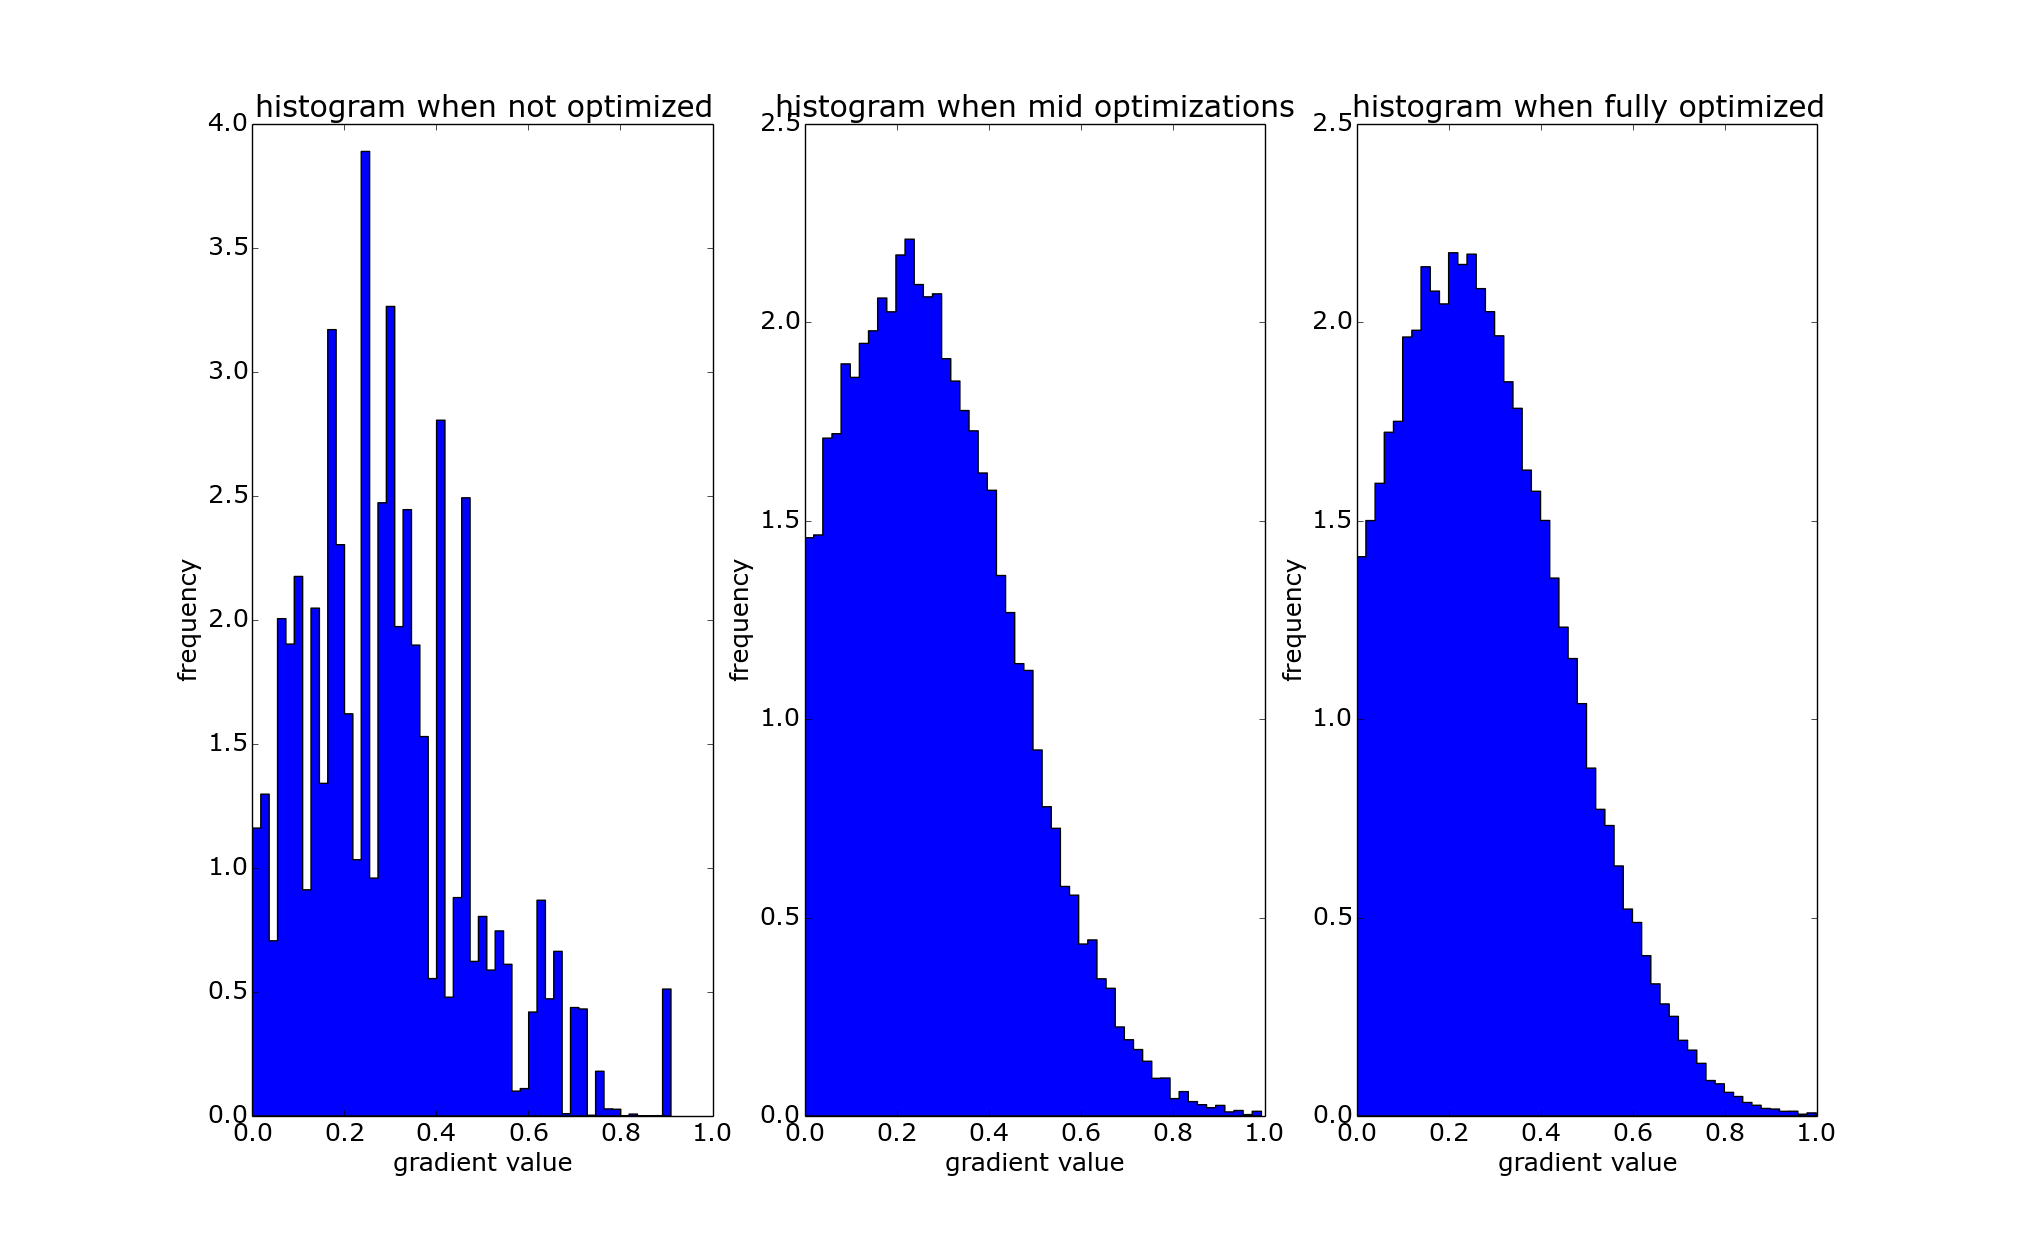
\includegraphics[width=16cm]{images/crickets.png}}

As you can see the first set of optimizations improve the sample quality greatly but do little to the running time. The second set of optimizations do little to the sample quality but improve the running time significantly.

We hope that this example has demonstrated and explained what it is that our compiler achieves and why there is a need for such a compiler.



%     ######       ######     ##     #####  ##   ##  #####   ######    #####  ##   ## ##    ## ###### 
%    ##    ##  ##  ##   ##   ####   ##   ## ##  ##  ##   ##  ##   ##  ##   ## ##   ## ###   ## ##   ##
%         ###  ##  ##   ##  ##  ##  ##      ## ##   ##       ##   ##  ##   ## ##   ## ####  ## ##   ##
%       ###        ######  ##    ## ##      ####    ##       ######   ##   ## ##   ## ## ## ## ##   ##
%     ###      ##  ##   ## ######## ##      ## ##   ##  #### ##  ##   ##   ## ##   ## ##  #### ##   ##
%    ##        ##  ##   ## ##    ## ##   ## ##  ##  ##   ##  ##   ##  ##   ## ##   ## ##   ### ##   ##
%    ########      ######  ##    ##  #####  ##   ##  #####   ##    ##  #####   #####  ##    ## ###### 

\section{Background}



%     ######        ## 
%    ##    ##      ### 
%         ###       ## 
%       ###         ## 
%     ###           ## 
%    ##        ##   ## 
%    ########  ##  ####

\subsection{Bayesian probability}

Bayesian probability is a branch of probability and logic that deals with making predictions about future events based off of our prior assumptions and the outcomes of current events.

We assume that the reader has knowledge of basic probability ideas. This includes conditional probability, the idea that if \(A\) and \(B\) are events then
\[\Pr(A | B) = \frac{\Pr(A \land B)}{\Pr(B)}\]
is the probability of \(A\) occurring given that \(B\) has already occurred.

The central theorem of Bayesian probability is Bayes theorem, which is as follows: for two events \(A\) and \(B\),
\[\Pr(A | B) = \frac{\Pr(B | A) \Pr(A)}{\Pr(B)}\]
This comes straight from the definition of conditional probability. However, whilst we will usually know \(\Pr(A)\) and \(\Pr(B | A)\) we usually will not know \(\Pr(B)\). Here we can apply a theorem called the Law of Total Probability, which is as follows: If \(A\) is an event and \(\mathcal B = \{B_i\}\) forms a finite or countable partition of the sample space, then
\[\Pr(A) = \sum_{B_i \in \mathcal B} \Pr(A | B_i) \Pr(B_i)\]
This works for continuous events as well: If \(A\) is an event and \(X\) is a continuous random variable, then
\[\Pr(A) = \int_{-\infty}^\infty \Pr(A | X = x) \Pr(X = x) dx\]
This leads to an extended version of Bayes theorem which is as follows: If \(B\) is an event and \(\mathcal A = \{A_i\}\) forms a partition of the sample space, then
\[\Pr(A_i | B) = \frac{\Pr(B | A_i) \Pr(A_i)}{\sum_{A_j \in \mathcal A} \Pr(B | A_j) \Pr(A_j)}\]
And the continuous version: If \(B\) is an event and \(X\) a continuous random variable, then
\[\Pr(X = x | B) = \frac{\Pr(B | X = x) \Pr(X = x)}{\int_{-\infty}^\infty \Pr(B | X = x') \Pr(X = x') dx'}\]
These theorems are central to the work we will do throughout this project.



%     ######        ###### 
%    ##    ##      ##    ##
%         ###           ###
%       ###           ###  
%     ###           ###    
%    ##        ##  ##      
%    ########  ##  ########

\subsection{Probabilistic programming}

Superficially a probabilistic programming language may appear to be just like a normal one. In fact one could say that if you've ever written a program that calls a random number generator then you've written a probabilistic program. Probabilistic programming languages do indeed make it easy to sample from various probability distributions by having them built in to the language, but they do much more than that as well. A probabilistic programming language allows you to condition the entire execution on some observed data. We will explain what we mean by that in the next few paragraphs.

For the sake of this explanation a good way of thinking about all programs would be to consider the distribution of outputs they produce. For completely deterministic programs they may only produce one possible output. Once you start using random number generators they produce a distribution over many values. What we're interested in is this distribution of outputs of the program which we call the posterior distribution.

There are a few ways to calculate this posterior distribution. One method is to run it many times to generate an approximation which gets closer to the true posterior the more you run it. This is the method used by both Anglican and Probabilistic-C \cite{Anglican, ProbabilisticC}. Another way is to use static analysis on the program to track the distributions through it and calculate the posterior precisely. An example of this exact method can be seen in a implementation of Church called Cosh \cite{Cosh}. The exact method is of course more accurate but also far more computationally expensive. As a result it can usually only be used on very simple programs. During this paper we will only consider the inexact method of inference.

Where things get more complicated is when we introduce the ability to observe. This is the true power of probabilistic programming languages. This allows you to condition the entire program execution on some observed data and change the posterior distribution to match.

Suppose we first sample a variable \(Y\) from a distribution. So we know \(\Pr(Y = y)\). Then suppose we observe a piece of data \(X\). So we know \(\Pr(X = x | Y = y)\). After the observe statement we expect the variable \(Y\) to instead follow the distribution \(\Pr(Y = y\ |\ X = x)\). It may not be possible to calculate this distribution analytically, but this is the purpose of the inference algorithm of the probabilistic programming language.

To illustrate the process, consider the following simple Anglican program.

\begin{center}
	\begin{varwidth}{\linewidth}
		\small
		\begin{verbatim}
			[assume p (uniform-continuous 0 1)]
			[observe (flip p) true]
			[predict p]
		\end{verbatim}
	\end{varwidth}
\end{center}
What this means in terms of probabilities is: \(\Pr(p) = 1\), \(\Pr(x | p) = p\). Then we expect the posterior distribution of \(p\) to be
\[\Pr(p | x) = \frac{\Pr(x | p) \Pr(p)}{\int_0^1 \Pr(x | p') \Pr(p') dp'} = 2p\]
and this is exactly the output we see if we run the program. Although we have done it here it is not in general possible to work out the conditional probability analytically. Probabilistic programming gives us the power to approximate any probability of this form whether or not we can't calculate it directly.

Now that we have a basic idea of the semantics of an observe statement, we will define two related but different types of observation and ways of doing inference on each.

What we will call a hard observation asserts the result of some non-probabilistic boolean expression. This is the way that Church handles observations. One way to do inference using this kind of observation is to simply run the program many times and restart from the beginning whenever you fail an observation. This way only traces which satisfy all the observations will make it to the end and be recorded. This is known as rejection sampling and is a rather unsophisticated and limited way of doing inference. There are other ways of doing inference using these observations but they are more complicated and it is not necessary to understand them here.

What we will call a soft observation instead samples from a probability distribution and asserts that it received a particular value. This is the way that both Anglican and Probabilistic-C handle observations. Now that we might be sampling continuous values from probability distributions we can't do rejection sampling anymore, instead we use particles. The basic idea is to run the same program many times in parallel where each individual instance of the program is called a particle. The particles are made to synchronize with each other at observe statements. A consequence of this is a prerequisite that all possible runs of the program must hit the same number of observe statements. When a particle comes to an observe statement it calculates the probability of that observation being satisfied. Once all particles have reached the observe statement the less likely particles may be killed off and new ones are cloned from those that remain to keep the number of particles constant. The end result is that the distribution of values of variables throughout the collection of particles converges to the correct posterior distribution.

This concludes our overview of probabilistic programming. Next we will describe the two languages Anglican and Probabilistic-C in more detail.



%     ######        ##### 
%    ##    ##      ##   ##
%         ###           ##
%       ###         ##### 
%     ###               ##
%    ##        ##  ##   ##
%    ########  ##   ##### 

\subsection{Anglican and Probabilistic-C}

Anglican and Probabilistic-C are the two established probabilistic programming languages that we'll be concentrating on. The source language of our compiler is based on Anglican and the target language of our compiler is Probabilistic-C.

Anglican is a high level probabilistic programming language based upon a subset of the language Lisp. The exact syntax is that it is a sequence of assume, observe, and predict directives. Each directive may then contain expressions which come from a safe, functional subset of Lisp. An assume directive defines a new identifier and can be thought of as a let expression. An observe directive performs a soft observation as we defined in the previous section. A predict directive prints out a value to the terminal. The Lisp subset used for the inner expressions includes all the basic flow control elements, lots of mathematical operators, and a large selection of probabilistic distributions to sample from. As we've said, Anglican is high level and this makes it nice to program in. However, for complex models it can be slow.

Probabilistic-C is a lower level probabilistic programming language based upon C. In fact the only difference is the addition of a library of sampling functions, two extra functions to observe and predict, and a macro which redefines the main function. This means that Probabilistic-C has all of the power of C and almost all of the speed. An observe statement in Probabilistic-C also performs a soft observation. These are the same semantics as in Anglican and this makes the compilation easier. If our source language was based on Church for example, then the compilation would be considerably harder as the semantics of observations would be different. Probabilistic-C is different from most probabilistic programming languages in that you are very unconstrained in your observations. In most languages you would be required to supply a distribution and a value to an observe statement. However, in Probabilistic-C you simply supply a floating point value representing the log of the probabilistic density function of the distribution at the desired point. This lack of restriction makes Probabilistic-C unsafe in the sense that you can write programs that make no sense statistically. However, we will use this extra power to do optimizations and it gives us a lot of options that we would not have with another target language. For this reason and C's general unfriendliness it is not recommended to code in Probabilistic-C directly. It does a perfect compilation target though.

Combine the facts about these two languages and you can see there is an obvious motive for creating a compiler between them.



%     #####        #####   #####  ##      ## ######  #### ##     ####### ######  
%    ##   ##  ##  ##   ## ##   ## ###    ### ##   ##  ##  ##     ##      ##   ## 
%         ##  ##  ##      ##   ## ####  #### ##   ##  ##  ##     ##      ##   ## 
%     #####       ##      ##   ## ## #### ## ######   ##  ##     ######  ######  
%         ##  ##  ##      ##   ## ##  ##  ## ##       ##  ##     ##      ##  ##  
%    ##   ##  ##  ##   ## ##   ## ##      ## ##       ##  ##     ##      ##   ## 
%     #####        #####   #####  ##      ## ##      #### ###### ####### ##    ##

\section{The compiler}



%     #####        ## 
%    ##   ##      ### 
%         ##       ## 
%     #####        ## 
%         ##       ## 
%    ##   ##  ##   ## 
%     #####   ##  ####

\subsection{The source language}

For this project we needed a high level probabilistic programming language to be the source language of our compiler. We had two choices: to use an existing one or to write our own. In fact we went somewhere in between by modifying Anglican to include some extra type information to make compilation easier. Compiling from an untyped language to a typed one is difficult. One way would be to forget the idea of using native types and introduce a layer of abstraction around all variables but this could incur a large performance penalty. We therefore made the choice to introduce some extra type information into our source language so that we always know the type of a variable or function argument or a function return type.

What follows are a couple of examples of our language. We will refer to our source language as G since the paper we are following by G. Morrisett et al. used a language named F \cite{SystemF}. This first example shows that G is identical to Anglican for programs not involving user-defined functions or lists.
\begin{center}
	\begin{varwidth}{\linewidth}
		\small
		\begin{verbatim}
			[assume iscloudy (flip 0.5)]
			
			[assume israining (if iscloudy (flip 0.8) (flip 0.2))]
			
			[assume sprinkler (if iscloudy (flip 0.1) (flip 0.5))]
			
			[assume pwetgrass (if (and sprinkler israining) 0.99
												(if (or  sprinkler israining) 0.9
																											0))]
			
			[observe (flip pwetgrass) true]
			
			[predict israining]
		\end{verbatim}
	\end{varwidth}
\end{center}
However for more complicated programs we need to add type information to the function arguments, function return type, and anywhere that something is extracted from a list. This second example demonstrates all of these.
\begin{center}
	\begin{varwidth}{\linewidth}
		\small
		\begin{verbatim}
			; Prior drill beliefs
			[assume state-of-nature (list 0.5 0.3 0.2)] 

			; Oil quantity: dry, wet or soaking (0, 1 or 2)
			[assume oil-quant (discrete state-of-nature)]

			; Sensor reliability conditional distribution
			[assume sound-state-dist (lambda (o : Num) -> List
				(cond ((= o 0) (list .6 .3 .1))
							((= o 1) (list .3 .4 .3))
							(else    (list .1 .4 .5))))]

			; Utility function 
			[assume utility (lambda (drill : Bool) -> Num 
				(if drill
						(nth Num (list -70 50 200) oil-quant)
						0))]

			; Make a sound observation
			[observe (discrete (sound-state-dist oil-quant)) 2]

			; Predict the oil quantity in the well
			[predict oil-quant]

			; What is the utility if we decide to drill?
			[predict (utility true)]

			; What is the utility if we don't?
			[predict (utility false)]

			; With what probability should I drill?
			[assume should-i-drill (if (> (utility true) (utility false)) 1 0)]
			[predict should-i-drill]
		\end{verbatim}
	\end{varwidth}
\end{center}
What follows is an exact description of the syntax of G.
\begin{center}
	\begin{varwidth}{\linewidth}
		\small
		\begin{verbatim}
			<program> ::= <directive> | <directive> <program>
			<directive> ::= "[" "assume" <id> <expr> "]" |
											"[" "observe" <expr> <expr> "]" |
											"[" "predict" <expr> "]"
			<exprs> ::= <expr> | <expr> <exprs>
			<expr> ::= <number> | <boolean> | <empty-list> | <id> |
								 <let-expr> |
								 <lambda-expr> | <mem-expr> |
								 <if-expr> | <cond-expr> |
								 <prim-expr> | <typed-prim-expr> |
								 <app-expr>
			<let-expr> ::= "(" "let" <id> <expr> <expr> ")"
			<lambda-expr> ::= "(" "lambda" <lambda-type> <expr> ")"
			<lambda-type> ::= "(" <lambda-args> ")" "->" <type>
			<lambda-args> ::= <id> ":" <type> | <id> ":" <type> <lambda-args>
			<mem-expr> ::= "(" "mem" <expr> ")"
			<if-expr> ::= "(" "if" <expr> <expr> <expr> ")"
			<cond-expr> ::= "( "cond" <cond-args> ")"
			<cond-args> ::= "(" "else" <expr> ")" |
											"(" <expr> <expr> ")" <cond-args>
			<prim-expr> ::= "(" <prim> <exprs> ")"
			<typed-prim-expr> ::= "(" <typed-prim> <type> <exprs> ")"
			<app-expr> ::= "(" <exprs> ")"
			<prim> ::= "+" | "-" | "*" | "/" |
								 "=" | "!=" | "<" | ">" | "<=" | ">=" |
								 "and" | "or" | "not" |
								 "list" | "cons" | "rest" | "empty" | "count" |
								 "log" | "log10" | "exp" |
								 "pow" | "sqrt" | "cbrt" |
								 "floor" | "ceil" | "round" | "rint" |
								 "abs" | "signum" |
								 "sin" | "cos" | "tan" |
								 "asin" | "acos" | "atan" |
								 "sinh" | "cosh" | "tanh" |
								 "inc" | "dec" | "mod" |
								 "flip" | "beta" | "gamma" | "normal" | "poisson" |
								 "geometric" | "exponential" |
								 "uniform-continuous" | "uniform-discrete" | "discrete"
			<typed-prim> ::= "first" | "second" | "nth" | "categorical"
			<types> ::= <type> | <type> "," <types>
			<type> ::= "Num" | "Bool" | "List" | "(" <types> ")" "->" <type>
		\end{verbatim}
	\end{varwidth}
\end{center}



%     #####        ###### 
%    ##   ##      ##    ##
%         ##           ###
%     #####          ###  
%         ##       ###    
%    ##   ##  ##  ##      
%     #####   ##  ########

\subsection{Typing the source language}

The first stage of compilation is to type the source language. We assign a type to every node of the abstract syntax tree (AST). Later on in the compiler we will reduce the type information we store to only remembering the types of identifiers. The typing itself is very easy as all the information is there and only minimal to no inference has to be done. The checks performed are:
\begin{itemize}
\item
	That all variables are defined before they are used.

\item
	For all built-in (untyped) primitives (e.g. \texttt{+}, \texttt{-}, \texttt{and}, \texttt{or}) we know their type or can give them one from their arguments. Then we just check that the types of the arguments match what we expected. What we mean by give them a type is that for example if \texttt{=} had 4 arguments and the first was a number, then we would give it the type
	\begin{verbatim}
		(Num, Num, Num, Num) -> Bool
	\end{verbatim}
	For functions such as \texttt{first} we also use the user supplied type. Often the user supplied type is used as the return type. It is worth noting that although in G the first argument of \texttt{first} appears to be a type that is not a true argument. A better way of thinking about it that it specifies which of a set of functions you're referring to.

\item
	That the given return type of a lambda matches the type that its body evaluates to. The reason for making the user specify a return type at all is for recursive functions so we don't have to do any type guesswork at all.

\item
	That the two branches of an if expression have the same type.

\item
	In a plain old application we use the map from expressions to types that we have built up to type each expression, we then check that the first expression is a function type and its argument types match the types of the rest of the expressions.

\item
	For an observe directive we check that the outer expression of the first argument is a probabilistic primitive. The list of probabilistic primitives is: \texttt{flip}, \texttt{beta}, \texttt{gamma}, \texttt{normal}, \texttt{poisson}, \texttt{geometric}, \texttt{exponential}, \texttt{uniform-continuous}, \texttt{uniform-discrete}, \texttt{discrete}, \texttt{categorical}.

\end{itemize}



%     #####        ###### 
%    ##   ##      ##    ##
%         ##            ##
%     #####        ###### 
%         ##            ##
%    ##   ##  ##  ##    ##
%     #####   ##   ###### 

\subsection{Making identifiers unique}

At this point in the compilation we change all identifiers to be unique. After this point whenever two identifiers are the same they always refer to the same variable. This means that we can work out scoping rules now and then never have to think about them again for the rest of the compilation. It also removes the complication that Lisp's list of characters allowed in identifiers is a lot larger than C's. This does have the downside that with all the names changed the outputted C harder to understand, but that is a price worth paying.



%     #####           ### 
%    ##   ##         #### 
%         ##        ## ## 
%     #####        ##  ## 
%         ##      ########
%    ##   ##  ##       ## 
%     #####   ##       ## 

\subsection{Into continuation passing style}

The next step of compilation is to transform into continuation passing style (CPS). The primary difference here is that functions and arithmetic operators and such like do not return values but instead take as an extra argument an explicit continuation. A continuation is a function of one argument which caries on the computation. The reason for doing this is that it makes explicit a lot of things that were originally implicit such as intermediate values and order of evaluation. This immediately brings the style of execution away from a functional language with nested expressions and more towards an imperative one where statements are executed in order. In other words it brings the style of execution a lot closer to that of C. The exception to the transformation is built-in primitives which we assume can be done atomically by the target language. Primitives can therefore be calculated directly and stored into variables.

We wont say too much about the actual transformation as it's fairly standard. The two points we will mention are:
\begin{itemize}
\item
	Generate the continuation for an if expression before and then use the same one in each branch instead of generating code within each branch. This has the effect of increasing the number of continuations but reduces the overall amount of code generated and reduces the nesting level.

\item
	When transforming a let expression of a lambda make sure that the resulting generated lambda is assigned to the correct id rather than to a new or temporary one. This is because the lambda could be recursive and we must make sure that it is assigned to the id it is expecting. 

\end{itemize}



%     #####       ########
%    ##   ##      ##      
%         ##      ##      
%     #####        ###### 
%         ##            ##
%    ##   ##  ##  ##    ##
%     #####   ##   ###### 

\subsection{Closure conversion and hoisting}

The goal of this step of compilation is to lift all functions to the top level of the program. This is because in C all functions must be defined in this way. The problem we must overcome is that functions may have free variables. What we mean by this is variables which are used in the function but not defined within it or one of the arguments. The way we will fix this is to effectively add more arguments to all functions so that they no longer contain any free variables. In practice however we keep the original arguments and add one new one. The way we do this is that whenever a function is created we store the values of all its free variables into some kind of bundle or closure. Then when the function is executed we unpack the bundle to get back the values of any free variable that are needed.

The first thing we do is to go though the entire program and through every function to find the free variables. We work out which variables are used in the function but not defined within it or one of the arguments. Once that is done we then make the following changes:
\begin{itemize}
\item
	The list of names and types of a function's free variables is added to the function definition and that definition is then lifted or hoisted to the top level. The function is also changed to accept as its first argument a bundle containing the free variables. When executed the first thing the function will do is to unpack the bundle into variables of the correct name and then it will execute its original body.

\item
	Where a function was originally defined we instead form a bundle containing the name of the function being called and a list of all its free variables.

\item
	Any invocations of functions will have to be changed to have a previously created bundle passed as the first argument.

\end{itemize}



%     #####           ## 
%    ##   ##         ##  
%         ##        ##   
%     #####        ##### 
%         ##      ##   ##
%    ##   ##  ##  ##   ##
%     #####   ##   ##### 

\subsection{Into C}

Before outputting C code we first do a final transformation into a C-like AST. We try to do as much of the calculation here to make the printing itself trivial. Most of the work is about allocating identifiers to bundles and making sure that they are packed and unpacked correctly.

We alter the idea of a bundle to be made of two parts. Firstly there is the part we will call the data. This contains the actual values of the free variables and is specific to a particular function. Then there is the part we will continue to call the bundle. This contains a pointer to the function to the executed and a pointer to a data object. Each bundle relates to a function signature (i.e. a function type). We create bundles and data objects in one pass though the code. We explicitly pack each individual free variable into a data object and explicitly unpack of variables from data objects at the start of functions.

One important point to make is that we do not try to do any explicit memory management. The main reason for this is that it is unnecessary. It is important to understand that the program execution happens within many short lived threads. As each thread dies all its allocated memory is freed by the operating system. Therefore as it is such a complex thing to do and the memory usage benefits are small we decide to not do explicit memory management.



%     #####       ########
%    ##   ##           ## 
%         ##          ##  
%     #####          ##   
%         ##        ##    
%    ##   ##  ##   ##     
%     #####   ##  ##      

\subsection{Outputting C code}

We need to output valid C code including struct definitions and any extra library functions used. Mostly the translation here is obvious and direct. The only difficult point is to make sure that all structs and functions are declared before they are defined to allow full recursion.

There are a few times that we need to add in some extra C code to provide an implementation of linked lists or an extra math function. Some optimizations also require observing the result of a specific calculation. To this end some C code has been written in files to be included in the output if needed. Usually this is done by checking to see if any of a set of primitive functions is used.



%        ###        #####  ######  ######## #### ##      ## #### ########    ##    ######## ####  #####  ##    ##  ##### 
%       ####   ##  ##   ## ##   ##    ##     ##  ###    ###  ##       ##    ####      ##     ##  ##   ## ###   ## ##     
%      ## ##   ##  ##   ## ##   ##    ##     ##  ####  ####  ##      ##    ##  ##     ##     ##  ##   ## ####  ## ##     
%     ##  ##       ##   ## ######     ##     ##  ## #### ##  ##     ##    ##    ##    ##     ##  ##   ## ## ## ##  ##### 
%    ########  ##  ##   ## ##         ##     ##  ##  ##  ##  ##    ##     ########    ##     ##  ##   ## ##  ####      ##
%         ##   ##  ##   ## ##         ##     ##  ##      ##  ##   ##      ##    ##    ##     ##  ##   ## ##   ###      ##
%         ##        #####  ##         ##    #### ##      ## #### ######## ##    ##    ##    ####  #####  ##    ##  ##### 

\section{Optimizations}

At this point we already have a standard compiler from a high level to a lower level language. This would be a good enough project in itself. However, there is potential for massive increases in both performance and the quality of samples though the combination of a few simple optimizations.

All the optimizations described here are performed immediately after CPS transformation. In this stage the syntax is at a good balance of simplicity and expressiveness. For example all expressions have been split up so we only calculate one primitive or application at a time. Also, lambdas are still in-line and so we don't have to worry about variable scope as much. It is however still often useful to know the full history of a variable. By which we mean exactly how it was calculated rather than just the last step. We therefore calculate this history before doing any optimizations and rebuild the information after each optimization is complete.



%        ###        ## 
%       ####       ### 
%      ## ##        ## 
%     ##  ##        ## 
%    ########       ## 
%         ##   ##   ## 
%         ##   ##  ####

\subsection{Non-probabilistic optimizations}

We do some standard non-probabilistic optimizations. None of these are technically necessary for the rest of the optimizations to work and some would be performed by the C compiler anyway. They still make our life a little easier however so that is why they are included here.



%        ###         ##        ## 
%       ####        ###       ### 
%      ## ##         ##        ## 
%     ##  ##         ##        ## 
%    ########        ##        ## 
%         ##   ##    ##   ##   ## 
%         ##   ##   ####  ##  ####

\subsubsection{Constant expression calculation}

Here we intend to optimize any primitive such as plus or times where all of the arguments are constant. We can easily calculate what the answer should be and set the id equal to that rather than applying a primitive.

For example we could do the following optimization
\optimization{
	\begin{array}{l}
		\texttt{let x = prim + 2 5 in} \\
		\texttt{...}
	\end{array}
}{
	\begin{array}{l}
		\texttt{let x = 7 in} \\
		\texttt{...}
	\end{array}
}
This can be extended to the case when only some of the arguments are constant. In this case we can't remove the whole primitive application but we can reduce the number of arguments and hence the complexity of it.

For example we could do the following optimization
\optimization{
	\begin{array}{l}
		\texttt{let x = ... in} \\
		\texttt{let y = prim + x 2 5 in} \\
		\texttt{...}
	\end{array}
}{
	\begin{array}{l}
		\texttt{let x = ... in} \\
		\texttt{let y = prim + x 7 in} \\
		\texttt{...}
	\end{array}
}
We can optimize all of the following when at least some of the arguments are constant:
\begin{center}
	\texttt{+}, \texttt{-}, \texttt{*}, \texttt{/}, \texttt{eq}, \texttt{neq}, \texttt{<}, \texttt{>}, \texttt{<=}, \texttt{>=}, \texttt{and}, \texttt{or}, \texttt{not}
\end{center}
This sort of optimization would definitely be performed by any half decent C compiler. We are likely not improving the performance of the final compiled program by doing this. The reason for doing it is it reduces the size and complexity of the generated Probabilistic-C code greatly. This makes the other stages of compilation faster and easier and also makes it easier for a human to scan and understand the outputted Probabilistic-C code.



%        ###         ##        ###### 
%       ####        ###       ##    ##
%      ## ##         ##            ###
%     ##  ##         ##          ###  
%    ########        ##        ###    
%         ##   ##    ##   ##  ##      
%         ##   ##   ####  ##  ########

\subsubsection{Merging multiple arithmetic expressions}

Another thing we can do with arithmetic expressions is to merge ones of the same sort together.

For example we could do the following optimization
\optimization{
	\begin{array}{l}
		\texttt{let x = ... in} \\
		\texttt{let y = prim + x 5 in} \\
		\texttt{let z = prim + y 8 in} \\
		\texttt{let w = prim + z -4 in} \\
		\texttt{...}
	\end{array}
}{
	\begin{array}{l}
		\texttt{let x = ... in} \\
		\texttt{let w = prim + x 9 in} \\
		\texttt{...}
	\end{array}
}
This is a case that comes up in compiled programs surprisingly often as it can be caused by other optimizations. By optimizing it away we reduce the final complexity of the Probabilistic-C.

Again this optimization would likely be performed by the C compiler anyway so the final compiled program is unchanged.



%        ###         ##        ###### 
%       ####        ###       ##    ##
%      ## ##         ##             ##
%     ##  ##         ##        ###### 
%    ########        ##             ##
%         ##   ##    ##   ##  ##    ##
%         ##   ##   ####  ##   ###### 

\subsubsection{Removing let expressions where the id is not used}

A very simple optimization is to remove any let expression where the variable being assigned to is never used later on in the program.

This optimization doesn't do much on its own as the user is unlikely to have written a program that doesn't use one of its variables. However, almost all of the other optimizations we do here will leave orphaned variables that this process will clean up.

This is an optimization that a C compiler potentially would not perform. This is because C is a language with side effects so just because a variable is never used does not mean that the process of calculating it did not change program state. In our language however variables are immutable and there is no state so it is safe to remove the unused variable.



%        ###         ##           ### 
%       ####        ###          #### 
%      ## ##         ##         ## ## 
%     ##  ##         ##        ##  ## 
%    ########        ##       ########
%         ##   ##    ##   ##       ## 
%         ##   ##   ####  ##       ## 

\subsubsection{Removing let expressions where an id is assigned to another id}

Another very simple optimization is to remove a variable when it is assigned to the value of another variable. We then change all references to the removed variable in the rest of the program to the variable it was assigned to.

For example we could do the following optimization
\optimization{
	\begin{array}{l}
		\texttt{let x = ... in} \\
		\texttt{let y = x in} \\
		\texttt{let z = prim + y 1 in}\\
		\texttt{...}
	\end{array}
}{
	\begin{array}{l}
		\texttt{let x = ... in} \\
		\texttt{let z = prim + x 1 in}\\
		\texttt{...}
	\end{array}
}
This optimization is admittedly rather inconsequential but we include it anyway.



%        ###         ##       ########
%       ####        ###       ##      
%      ## ##         ##       ##      
%     ##  ##         ##        ###### 
%    ########        ##             ##
%         ##   ##    ##   ##  ##    ##
%         ##   ##   ####  ##   ###### 

\subsubsection{Removing trivial continuations}

The final non-probabilistic optimization we do it to remove trivial functions which are equivalent to another function. The place where this happens a lot is continuations generated from the translation into CPS.

For example we could do the following optimization
\optimization{
	\begin{array}{l}
		\texttt{let f = lambda x y z -> g x y z in} \\
		\texttt{...}
	\end{array}
}{
	\begin{array}{l}
		\texttt{let f = g in} \\
		\texttt{...}
	\end{array}
}
This will then of course be removed on the next pass as it is an id assigned to another id.

This optimization could be moderately important for performance. It's true that a decent C compiler will inline a small function such as the above and hence remove the extra application. The problem is that after the other transformations that we perform it will not be as simple so removing it at this stage will greatly simplify later stages of compilation.



%        ###        ###### 
%       ####       ##    ##
%      ## ##            ###
%     ##  ##          ###  
%    ########       ###    
%         ##   ##  ##      
%         ##   ##  ########

\subsection{Samples}

One of the things we'd like to do is to reduce the number of samples as some of them can be quite costly. We can also improve the quality of the ones we do. By this we mean we'd like to have a high level of mixing. We would therefore need to make fewer runs of the program before the output has converged enough towards to the correct output.



%        ###        ######         ## 
%       ####       ##    ##       ### 
%      ## ##            ###        ## 
%     ##  ##          ###          ## 
%    ########       ###            ## 
%         ##   ##  ##        ##    ## 
%         ##   ##  ########  ##   ####

\subsubsection{Merging samples}

One way we can improve performance is to reduce the number of samples as some of them can be moderately costly to perform. The ideal case for this optimization is shown below.
\[
	\begin{array}{l}
		\texttt{[assume x\_1 (normal m\_1 b\_1)]} \\
		\texttt{...} \\
		\texttt{[assume x\_n (normal m\_n b\_n)]} \\
		\texttt{[assume y (+ x\_1 ...\ x\_n)]}
	\end{array}
\]
The general form is where we make many samples and perform some function on them. We then use that function output and never use the individual samples anywhere else.

Assuming that none of the \texttt{x\_i} are used anywhere else then the above can be optimized into the following
\[
	\texttt{[assume y (normal (+ m\_1 ...\ m\_n) (+ b\_1 ...\ b\_n))]}
\]
We can even perform this optimization in the case where some of the \texttt{x\_i}s are used again. If only \texttt{x\_1} were used elsewhere then we could optimize to the following
\[
	\begin{array}{l}
		\texttt{[assume x\_1 (normal m\_1 b\_1)]} \\
		\texttt{[assume t (normal (+ m\_2 ...\ m\_n) (+ b\_2 ...\ b\_n))]} \\
		\texttt{[assume y (+ x\_1 t)]}
	\end{array}
\]
Although less of an optimization we have still reduced the number of samples.

There are many cases where we can apply this optimization and we have listed some of them below. We have only included here a few for the normal distribution, but the optimization can be applied to many other distributions and operations.

\begin{center}
	\resizebox{\textwidth}{!}{%
	\begin{tabular}{lcl}
		Before optimization && After optimization \\[2mm]
		\hline \\[-2mm]

		\(\begin{array}{l}
				\texttt{[assume x\_1 (normal m\_1 b\_1)]} \\
				\texttt{...} \\
				\texttt{[assume x\_n (normal m\_n b\_n)]} \\
				\texttt{[assume y (+ x\_1 ...\ x\_n)]}
			\end{array}\)
		&\(\Rightarrow\)&
		\texttt{[assume y (normal (+ m\_1 ...\ m\_n) (+ b\_1 ...\ b\_n))]} \\[15mm]

		\(\begin{array}{l}
				\texttt{[assume x\_1 (normal m\_1 b\_1)]} \\
				\texttt{...} \\
				\texttt{[assume x\_n (normal m\_n b\_n)]} \\
				\texttt{[assume y (- x\_1 ...\ x\_n)]}
			\end{array}\)
		&\(\Rightarrow\)&
		\texttt{[assume y (normal (- m\_1 ...\ m\_n) (+ b\_1 ...\ b\_n))]}

	\end{tabular}}
\end{center}
We will also prove the correctness of the first example.

\begin{mdframed}
	\begin{claim}
		The sum of independent normally distributed variables is normally distributed.
	\end{claim}
	\begin{claimproof}
		The easiest way to do this is using characteristic functions. For a random variable \(X\) this is

		\[\varphi_X(t) = E(e^{itX})\]
		The characteristic function of a normal distribution with mean \(\mu\) and variance \(\sigma^2\) is

		\[\varphi(t) = \exp(i t \mu - \frac{\sigma^2 t^2}{2})\]
		The characteristic function of the sum of two independent random variables \(X\) and \(Y\) is the product of their separate characteristic functions. Hence if \(X\) and \(Y\) are both normally distributed with means and variances \(\mu_X\), \(\mu_Y\) and \(\sigma_X^2\), \(\sigma_Y^2\) respectively then

		\begin{align*}
			\varphi_{X+Y}(t)
			& = \varphi_X(t) \varphi_Y(t) \\
			& = \exp\left(i t \mu_X - \frac{\sigma_X^2 t^2}{2}\right) \exp\left(i t \mu_Y - \frac{\sigma_Y^2 t^2}{2}\right) \\
			& = \exp\left(i t (\mu_x + \mu_Y) - \frac{(\sigma_X^2 + \sigma_Y^2) t^2}{2}\right)
		\end{align*}
		Which is the characteristic function of a normal distribution with mean \(\mu_X + \mu_Y\) and variance \(\sigma_X^2 + \sigma_Y^2\).

		From here if we have \(n\) independent normally distributed random variables \(X_i \sim N(\mu_i, \sigma_i^2)\) then we proceed by induction using the above to get that

		\[\sum_{i=1}^n X_i \sim N(\sum_{i=1}^n \mu_i, \sum_{i=1}^n \sigma_i^2)\]
	\end{claimproof}
\end{mdframed}



%        ###        ######         ###### 
%       ####       ##    ##       ##    ##
%      ## ##            ###            ###
%     ##  ##          ###            ###  
%    ########       ###            ###    
%         ##   ##  ##        ##   ##      
%         ##   ##  ########  ##   ########

\subsubsection{Doing arithmetic on samples}

Another thing we can do is merge some arithmetic operations into the sample as shown below. Although not very helpful at all on its own the hope is it would allow us to later merge more samples as in the previous optimization. With these two optimizations together we can merge any linear combination of samples into only one sample.

Here are some examples of the sort of optimizations we could do. However note that there are many others of this form that could be done and not just involving the normal distribution.

\begin{center}
	\resizebox{\textwidth}{!}{%
	\begin{tabular}{lcl}
		Before optimization && After optimization \\[2mm]
		\hline \\[-2mm]

		\(\begin{array}{l}
				\texttt{[assume x (normal m b)]} \\
				\texttt{[assume y (+ x r)]}
			\end{array}\)
		&\(\Rightarrow\)&
		\texttt{[assume y (normal (+ m r) b)]} \\[10mm]

		\(\begin{array}{l}
				\texttt{[assume x (normal m b)]} \\
				\texttt{[assume y (* x s)]}
			\end{array}\)
		&\(\Rightarrow\)&
		\texttt{[assume y (normal (* m s) (* b s s))]}

	\end{tabular}}
\end{center}



%        ###        ######        ###### 
%       ####       ##    ##      ##    ##
%      ## ##            ###            ##
%     ##  ##          ###         ###### 
%    ########       ###                ##
%         ##   ##  ##        ##  ##    ##
%         ##   ##  ########  ##   ###### 

\subsubsection{Pushing samples back}

Something we can do which has the capacity to greatly improve the quality of samples made is to move samples after potentially costly observe statements. The idea is that when an observe is made that kills almost all of the particles the ones which remain will all have been cloned from some small set and hence all samples that have been made also come from some small set. However, by moving the sample after the observe we can ensure that all particles have a different value of the sample just made whatever happens with the cloning of particles.

An example of what we might do is
\optimization{
	\begin{array}{l}
		\texttt{[assume x (poisson 1)]} \\
		\texttt{[assume y (normal 0 1)]} \\
		\texttt{[observe (normal x 1) 100]} \\
		\texttt{[predict y]}
	\end{array}
}{
	\begin{array}{l}
		\texttt{[assume x (poisson 1)]} \\
		\texttt{[observe (normal x 1) 100]} \\
		\texttt{[assume y (normal 0 1)]} \\
		\texttt{[predict y]}
	\end{array}
}
The only check we make when pushing samples back is whether the operation immediately following the samples uses the sampled value. If not then we move the sample past. Note that for this example we could potentially remove the observe and the value \texttt{x} completely as they have no effect on the predicted value \texttt{y}. However we do not consider this as in general it is hard to work out when it is safe to do so.

Care must be taken when implementing this so as to not end up in an infinite loop. For example where you are swapping two samples back and forth forever. The crucial point when implementing this therefore is to avoid just swapping with another sample.

So with that in mind, to push a sample back we scan from its position considering each statement encountered in the following manner:
\begin{itemize}
\item
	Suppose the statement depends on the sampled value. Then the sample cannot be moved back any further.

\item
	Suppose the statement is a \texttt{let} expression defining a new variable that does not depend on the sampled value. Then just ignore it and move on to the next statement.

\item
	Suppose the statement does depend on the sampled value and is not a \texttt{let} expression. Then the original sample is moved to be right after this statement. The process is then started again from the sample's new position.

\end{itemize}
This process is run repeatedly for every sample until no more changes can be made.



%        ###        ###### 
%       ####       ##    ##
%      ## ##             ##
%     ##  ##        ###### 
%    ########            ##
%         ##   ##  ##    ##
%         ##   ##   ###### 

\subsection{Merging of observe statements}

In most cases it is the observations that govern running time rather than any computation being performed, so much so that the cost of sampling and other computation is often negligible. Observations also impact on sample quality by causing the death and cloning of particles. This set of optimizations focus on merging observations together and can improve the speed of a program greatly.



%        ###        ######        ## 
%       ####       ##    ##      ### 
%      ## ##             ##       ## 
%     ##  ##        ######        ## 
%    ########            ##       ## 
%         ##   ##  ##    ##  ##   ## 
%         ##   ##   ######   ##  ####

\subsubsection{Merging observes of the same distribution}

The scenario here is that there are multiple consecutive observes of the same distribution. What we note is that it is usually the case then that their conjunction can be written in a nicer form. Often it can be written as a function of some selection of properties of the observed data such as the sum or the sample mean and variance.

This optimization can be applied to many different distributions. Some are obvious such as multiple identical Bernoulli observes being equivalent to one binomial observe. Some are more complicated such as the case of normal distributions which we will focus on.

If we have the situation
\[
	\begin{array}{l}
		\lbrack \mathsf{observe}\ (\mathsf{normal}\ m\ b)\ x_1 \rbrack \\
		\dots \\
		\lbrack \mathsf{observe}\ (\mathsf{normal}\ m\ b)\ x_n \rbrack
	\end{array}
\]
then we can show that it is equivalent to an observe that only relies on the sample mean and variance of the \(x_i\)'s. Note however that the resulting observe will not be of a normal distribution. In fact it will not be of any of the distributions that Probabilistic-C has a primitive for.

To work out what distribution it will have we consider the joint probability density function. This can be written as a product of the individual densities as all the observations are independent. Here \(\bar{x}\) denotes the sample mean and \(s^2\) the sample variance.

\begin{flalign*}
		 & \prod_{i=1}^n \frac{1}{\sqrt{2 \pi \sigma^2}} e^{-\frac{(x_i - \mu)^2}{2 \sigma^2}} & \notag\\
	=\ & (2 \pi \sigma^2)^{-\frac{n}{2}} e^{-\frac{1}{2 \sigma^2} \sum_{i=1}^n (x_i - \mu)^2} \notag\\
	=\ & (2 \pi \sigma^2)^{-\frac{n}{2}} e^{-\frac{1}{2 \sigma^2} \sum_{i=1}^n ((x_i - \bar{x}) - (\mu - \bar{x}))^2} \notag\\
	=\ & (2 \pi \sigma^2)^{-\frac{n}{2}} e^{-\frac{1}{2 \sigma^2} (\sum_{i=1}^n (x_i - \bar{x})^2 + \sum_{i=1}^n (\mu - \bar{x})^2 - 2 \sum_{i=1}^n (x_i - \bar{x})(\mu - \bar{x}))} \notag\\
		& \text{Then since }\sum_{i=1}^n (x_i - \bar{x})(\mu - \bar{x}) = 0 \notag\\
	=\ & (2 \pi \sigma^2)^{-\frac{n}{2}} e^{-\frac{1}{2 \sigma^2} (\sum_{i=1}^n (x_i - \bar{x})^2 + \sum_{i=1}^n (\mu - \bar{x})^2)} & \notag\\
	=\ & (2 \pi \sigma^2)^{-\frac{n}{2}} e^{-\frac{1}{2 \sigma^2} \sum_{i=1}^n (x_i - \bar{x})^2} e^{-\frac{n}{2 \sigma^2} (\mu - \bar{x})^2} \notag\\
	=\ & (2 \pi \sigma^2)^{-\frac{n}{2}} e^{-\frac{n - 1}{2 \sigma^2} s^2} e^{-\frac{n}{2 \sigma^2} (\mu - \bar{x})^2} \notag
\end{flalign*}

And importantly for us
\begin{flalign*}
		 & \log(\prod_{i=1}^n \frac{1}{\sqrt{2 \pi \sigma^2}} e^{-\frac{(x_i - \mu)^2}{2 \sigma^2}}) & \notag\\
	=\ & - \frac{n}{2} \log(2 \pi \sigma^2) - \frac{n - 1}{2 \sigma^2} s^2 - \frac{n}{2 \sigma^2} (\mu - \bar{x})^2 \notag
\end{flalign*}
We can then replace the sequence of observes or normal distributions by one observe of a function which calculates the above. This is the first optimization that is only possible within Probabilistic-C. This is because you are not limited to observing a standard builtin distribution but can pass any numerical value you want to an observe statement.



%        ###        ######        ###### 
%       ####       ##    ##      ##    ##
%      ## ##             ##           ###
%     ##  ##        ######          ###  
%    ########            ##       ###    
%         ##   ##  ##    ##  ##  ##      
%         ##   ##   ######   ##  ########

\subsubsection{Merging any consecutive observes}

This optimization relies on the way that observing works in Probabilistic-C. It is specific to Probabilistic-C and might not be possible in any other probabilistic programming language. This makes it rather interesting to us. The way that Probabilistic-C observes work is that you call the observe function with the log of the probability of the event happening. For all the standard distributions this relates to the log of the probability density function at that point but the crucial point is that we're not limited to named distributions. We can pass any floating point value to the observe function.

We therefore perform the following optimization
\optimization{
	\begin{array}{l}
		\texttt{observe(dist\_1(args\_1));} \\
		\texttt{...} \\
		\texttt{observe(dist\_1(args\_2));}
	\end{array}
}{
	\texttt{observe(}\sum_{i=1}^n\texttt{dist\_i(args\_i));}
}

This reduces the number of observe statements and gives us a large performance increase with no down side.



%        ###           ### 
%       ####          #### 
%      ## ##         ## ## 
%     ##  ##        ##  ## 
%    ########      ########
%         ##   ##       ## 
%         ##   ##       ## 

\subsection{Removal of observe statements}

The best way of improving both performance and mixing is to remove observe statements completely. That is what we try to do here.



%        ###           ###        ## 
%       ####          ####       ### 
%      ## ##         ## ##        ## 
%     ##  ##        ##  ##        ## 
%    ########      ########       ## 
%         ##   ##       ##   ##   ## 
%         ##   ##       ##   ##  ####

\subsubsection{Commuting samples and observe statements}

In certain cases we can compute the effect that an observe will have on a sample directly. We can then make those changes to the sample and potentially remove the observe. The term for what we're doing here is conjugate prior and there is a lot of statistical literature on the subject.

As an example we could perform the two following optimizations
\optimization{
	\begin{array}{l}
		\texttt{[assume p (beta a b)]} \\
		\texttt{[observe (flip p) true]}
	\end{array}
}{
	\texttt{[assume p (beta (+ a 1) b)]}
}

\optimization{
	\begin{array}{l}
		\texttt{[assume m (normal 3 1)]} \\
		\texttt{[observe (normal m 1) 6]}
	\end{array}
}{
	\texttt{[assume m (normal 4.5 0.5)]}
}
These are for the simple cases where the variable \texttt{a}, \texttt{b}, \texttt{m} are constants. If they are not then we might not be able to remove the observe completely as I explain later. This optimization has potential for huge increases in both performance and sample quality and could make it possible to write program which we infeasible before.

I will now give a proof of correctness for the first example in order to show what happens when parameters are unknown. Suppose we have the scenario as in the first example. This corresponds to having random variables \(p \sim Beta(\alpha, \beta)\) and \(x \sim Bernoulli(p)\), so \(\text{P}(p) = \frac{p^{\alpha - 1} (1 - p)^{\beta - 1}}{\text{B}(\alpha, \beta)}\) and \(\text{P}(x\ |\ p) = p\).

By Bayes theorem
\begin{flalign*}
		 \text{P}(p\ |\ x)
	&= \frac{\text{P}(x\ |\ p) \text{P}(p)}{\text{P}(x)}
	 = \frac{\text{P}(x\ |\ p) \text{P}(p)}{\int_0^1 \text{P}(x\ |\ p') \text{P}(p') dp'} \\
	&= \frac{\frac{p^\alpha (1 - p)^{\beta - 1}}{\text{B}(\alpha, \beta)}}{\int_0^1 \frac{p'^\alpha (1 - p')^{\beta - 1}}{\text{B}(\alpha, \beta)} dp'} \\
	&= \frac{p^\alpha (1 - p)^{\beta - 1}}{\int_0^1 p'^\alpha (1 - p')^{\beta - 1} dp'} \\
	&= \frac{p^\alpha (1 - p)^{\beta - 1}}{\text{B}(\alpha + 1, \beta)}
\end{flalign*}
Hence \(p\ |\ x \sim Beta(\alpha + 1, \beta)\). Then what's left is
\begin{flalign*}
		 \text{P}(x)
	&= \int_0^1 \text{P}(x\ |\ p') \text{P}(p') dp' \\
	&= \int_0^1 \frac{p'^\alpha (1 - p')^{\beta - 1}}{\text{B}(\alpha, \beta)} dp' \\
	&= \frac{\text{B}(\alpha + 1, \beta)}{\text{B}(\alpha, \beta)} \\
	&= \frac{\alpha}{\alpha + \beta}
\end{flalign*}
Thus as \(\text{P}(x\ |\ p) \text{P}(p) = \text{P}(x) \text{P}(p\ |\ x)\) we can replace the sample to be from the \(Beta(\alpha + 1, \beta)\) distribution and the observe to be of the value \(\frac{\alpha}{\alpha + \beta}\).

If \(\alpha\) and \(\beta\) are constant then this observe can then be removed entirely as is explained in the next optimization. If not then the observe must remain.

Note that the observe is no longer one of Anglican's distributions and so the optimization cannot be performed within Anglican. However, within Probabilistic-C or our intermediate language we can observe any distribution we like or even just numeric values.

I will also detail here the formula used for the conjugate prior of the normal distribution. With this optimization it is possible to go beyond merely the example given but instead to have the mean of the observed normal distribution be some linear function of a normally sampled variable. Suppose we have the following scenario
\[
	\begin{array}{l}
		\texttt{[assume m\_2 (normal m\_1 b\_1)]} \\
		\texttt{[observe (normal (+ (* m\_1 coeff) const) b\_2) v]}
	\end{array}
\]
Then they can be replaced by
\[
	\begin{array}{l}
		\texttt{[assume m\_2 (normal nm\_1 nb\_1)]} \\
		\texttt{[observe (normal nm\_2 nb\_2) v]}
	\end{array}
\]
where
\begin{flalign*}
	\texttt{nm\_1} &= \left( \frac{1}{\texttt{b\_1}} + \frac{\texttt{coeff}^2}{\texttt{b\_2}} \right)^{-1} \left( \frac{\texttt{m\_1}}{\texttt{b\_1}} + \frac{\texttt{coeff}}{\texttt{b\_2}} \left( \texttt{v} - \texttt{const} \right) \right) \\
	\texttt{nb\_1} &= \left( \frac{1}{\texttt{b\_1}} + \frac{\texttt{coeff}^2}{\texttt{b\_2}} \right)^{-1} \\
	\texttt{nm\_2} &= \texttt{coeff} \times \texttt{m\_1} + \texttt{const} \\
	\texttt{nb\_2} &= \texttt{b\_1} \times \texttt{coeff}^2
\end{flalign*}
Again if \texttt{m\_1} and \texttt{b\_1} are constant then the observe can be removed completely. If not then observe is at least no longer dependent on the value \texttt{m\_2} and this is a huge improvement. It is possible to remove any normal observe whose mean is a linear combination of any number of other normally sampled variables with constant parameters.



%        ###           ###        ###### 
%       ####          ####       ##    ##
%      ## ##         ## ##            ###
%     ##  ##        ##  ##          ###  
%    ########      ########       ###    
%         ##   ##       ##   ##  ##      
%         ##   ##       ##   ##  ########

\subsubsection{Removal of constant observe statements}

Here the idea is that if all of the arguments to an observe statement are constant then that observe can have no influence on the posterior distribution. In this case we we can remove the observe and not change the posterior distribution. The reason for this is that the distribution used to allocate children to the particles is uniform. This does not mean that every particle gets precisely one child, but averaging over many iterations the posterior distribution is unchanged. Removing the observe will increase performance and will also increase the quality of the samples produced. The reason for increasing sample quality is to do with unique particles. At an observe some particles are killed and others are cloned. This results in a decrease in the total number of unique particles. Therefore by not doing the observe we keep the number of unique particles as high as possible.



%    ########      ######## #######  #####  ########        ######      ##    ########    ##   
%    ##        ##     ##    ##      ##         ##           ##   ##    ####      ##      ####  
%    ##        ##     ##    ##      ##         ##           ##   ##   ##  ##     ##     ##  ## 
%     ######          ##    ######   #####     ##           ##   ##  ##    ##    ##    ##    ##
%          ##  ##     ##    ##           ##    ##           ##   ##  ########    ##    ########
%    ##    ##  ##     ##    ##           ##    ##           ##   ##  ##    ##    ##    ##    ##
%     ######          ##    #######  #####     ##           ######   ##    ##    ##    ##    ##

\section{Experimental data}

Here I will show to you with experimental data just how much benefit the different optimizations can give. For each one I will usually show both how it affects performance and mixing, that is how quickly we can make samples and how quickly those samples converge to the correct posterior distribution.



%    ########       ## 
%    ##            ### 
%    ##             ## 
%     ######        ## 
%          ##       ## 
%    ##    ##  ##   ## 
%     ######   ##  ####

\subsection{Pushing samples backwards}

To test this optimization I used a program of the following form.

\[
	\begin{array}{l}
		\texttt{[assume x (normal 0 1)]} \\
		\texttt{[assume y (poisson 1)]} \\
		\texttt{[observe (normal y 0.1) v]} \\
		\texttt{[predict x]}
	\end{array}
\]
Where the value of \texttt{v} can be varied. Programs of the above form were compiled with either no optimizations enabled or all optimizations enabled. The resulting programs were then run for 1000 iterations with 100 particles.

I will show the resulting histograms and a visualization of how quickly it converges to the final posterior distribution. I should point out that the running time of the optimized and non-optimized programs is identical.

First consider the case of \texttt{v = 3}, as shown in the following graphs.

\centerline{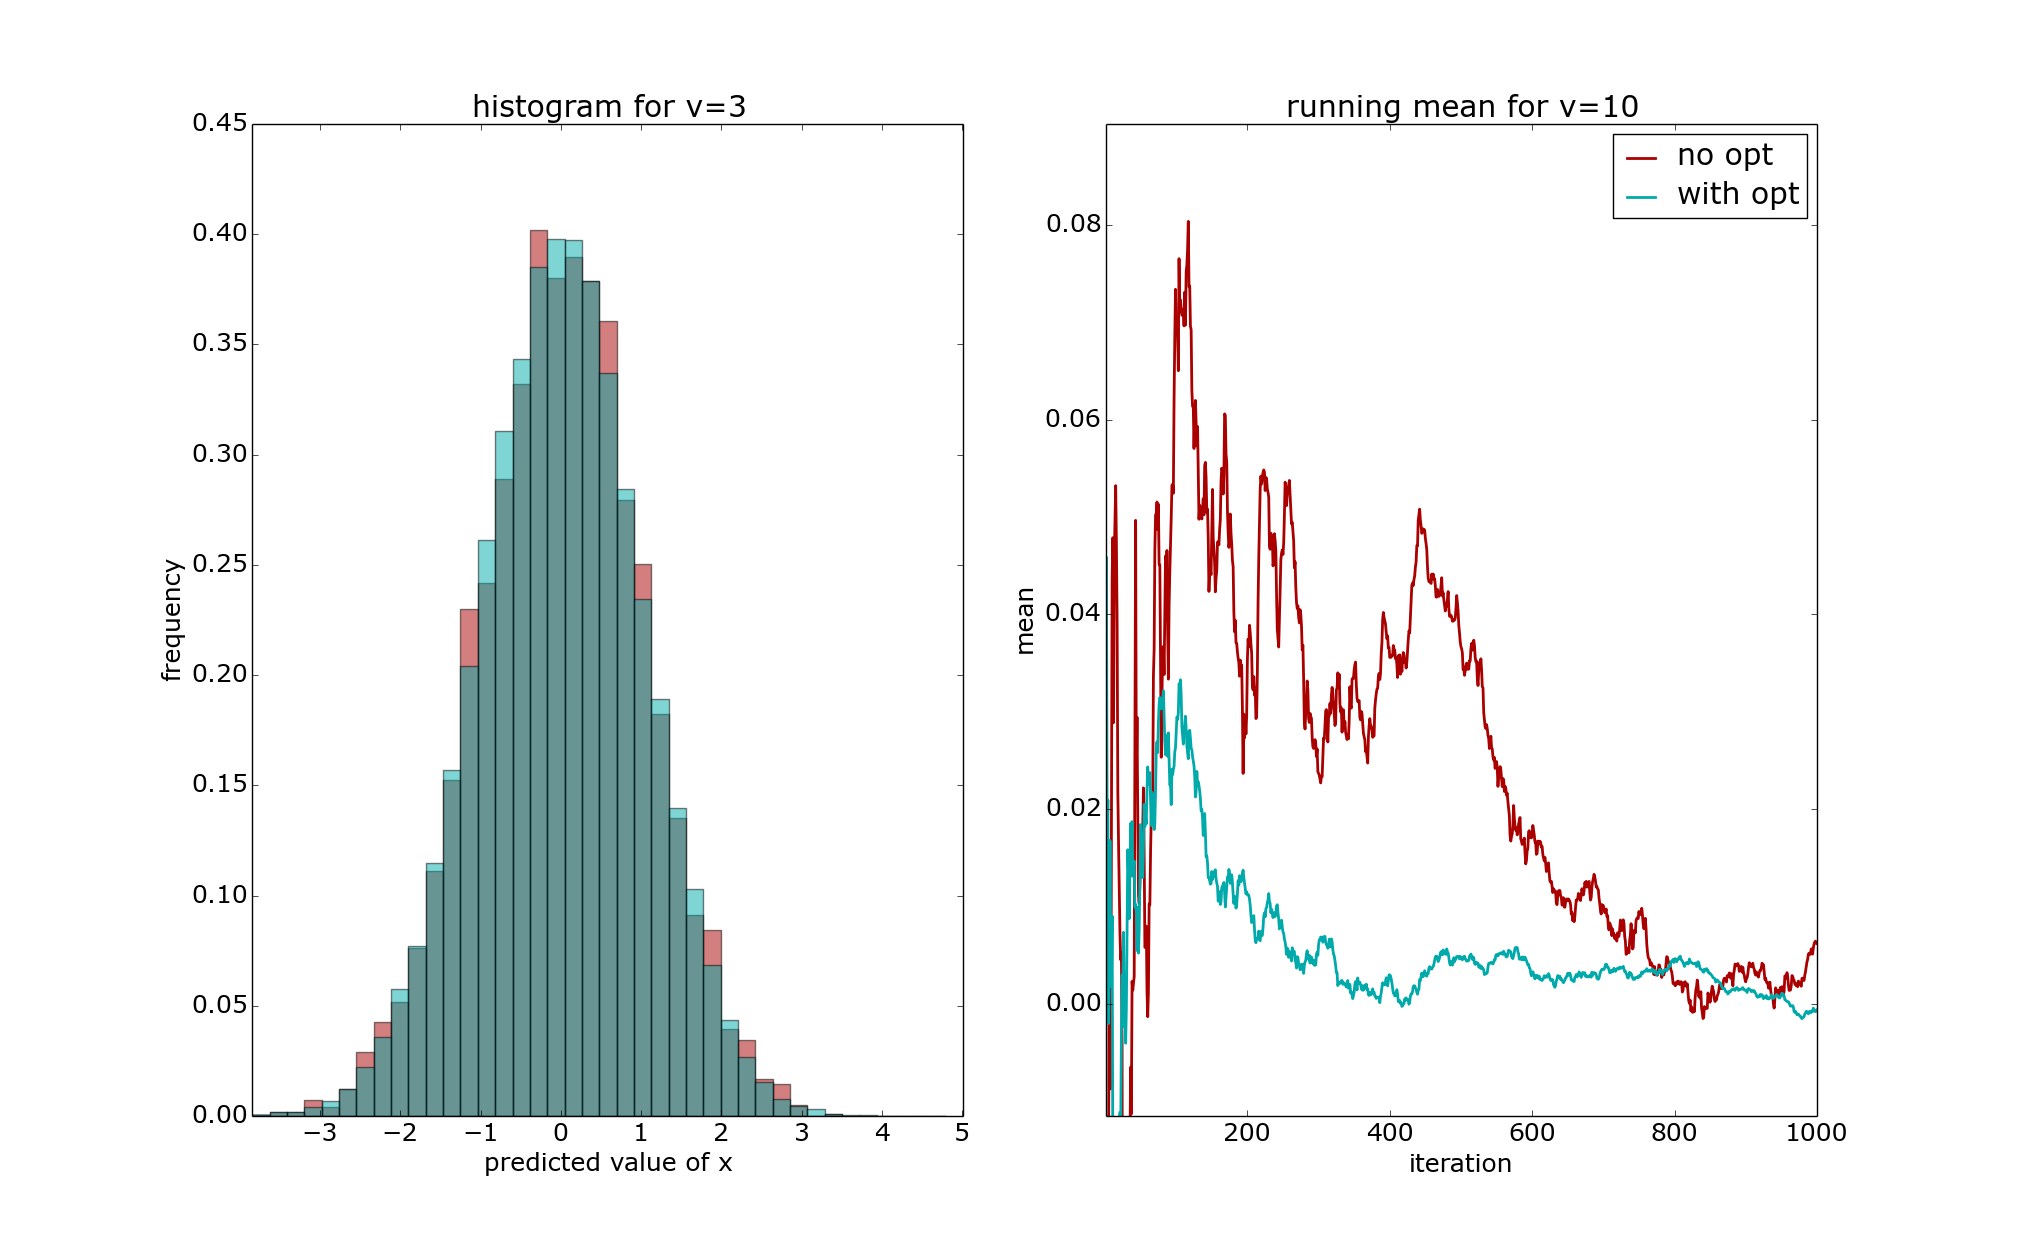
\includegraphics[width=16cm]{images/pushing_samples_back_1.png}}

This case demonstrates when the non-optimized program is still usable but the optimized program is superior in its mixing.

Now consider instead the case of \texttt{v = 10}, as shown in the next two graphs.

\centerline{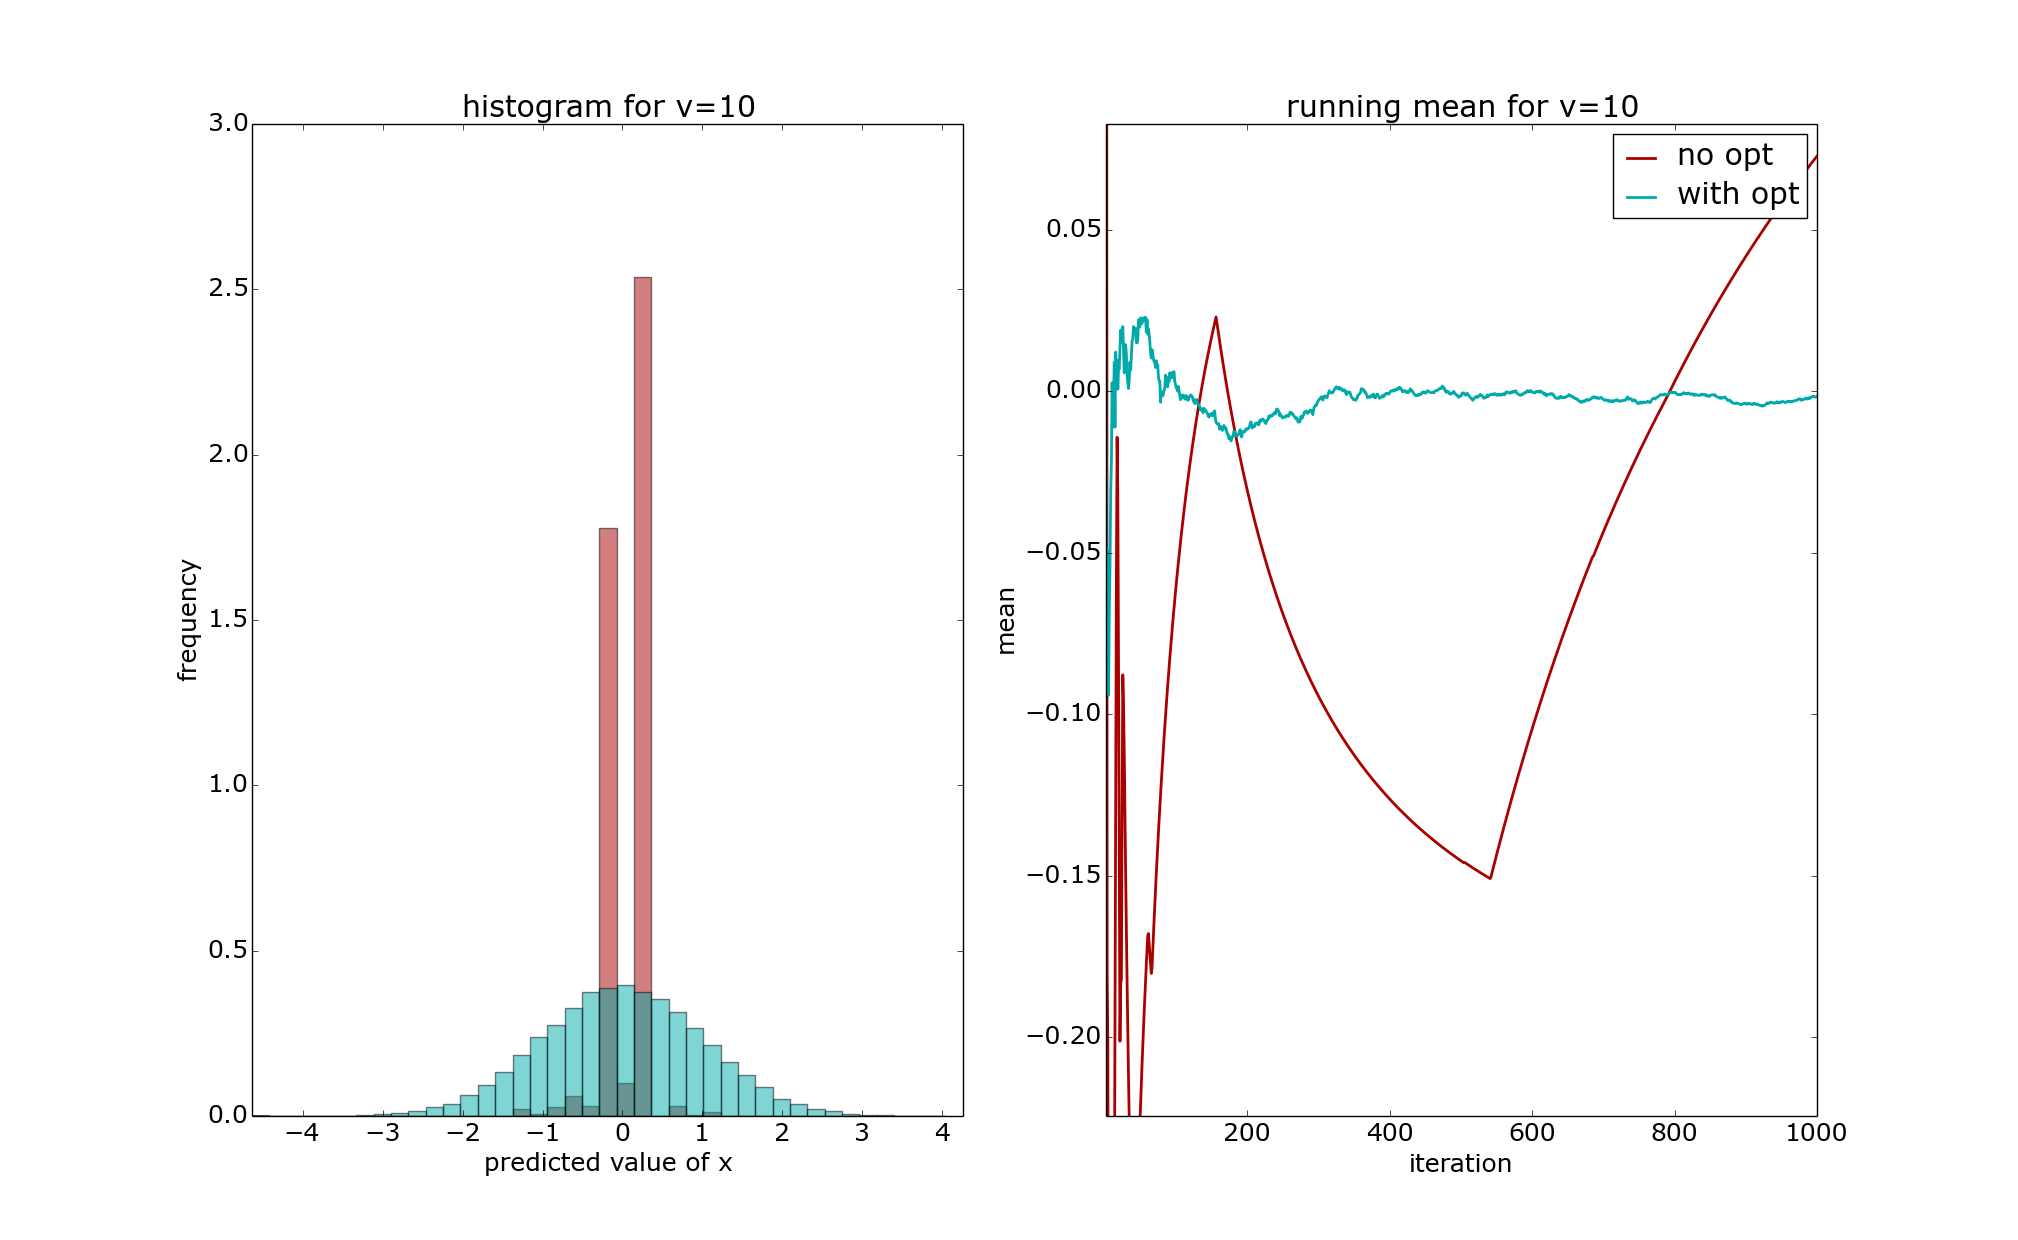
\includegraphics[width=16cm]{images/pushing_samples_back_2.png}}

This case demonstrates when the non-optimized program is completely useless however the optimized program is working exactly as well as it was before.



%    ########       ###### 
%    ##            ##    ##
%    ##                 ###
%     ######          ###  
%          ##       ###    
%    ##    ##  ##  ##      
%     ######   ##  ########

\subsection{Merging observes of the same distribution}

To test this optimization I used a program of the following form.

\[
	\begin{array}{l}
		\texttt{[assume m (poisson 40)]} \\
		\texttt{[assume b 20]} \\
		\texttt{[observe (normal m b) 45]} \\
		\texttt{...} \\
		\texttt{[observe (normal m b) 45]} \\
		\texttt{[predict m]}
	\end{array}
\]
Where the number of observe statements was varied. Programs of the above form were compiled with either no optimizations enabled or all optimizations enabled. The resulting programs were then run for 1000 iterations with 100 particles.

The following two graphs show running time against number of observes and mean value of the posterior distribution against number of observes.

\centerline{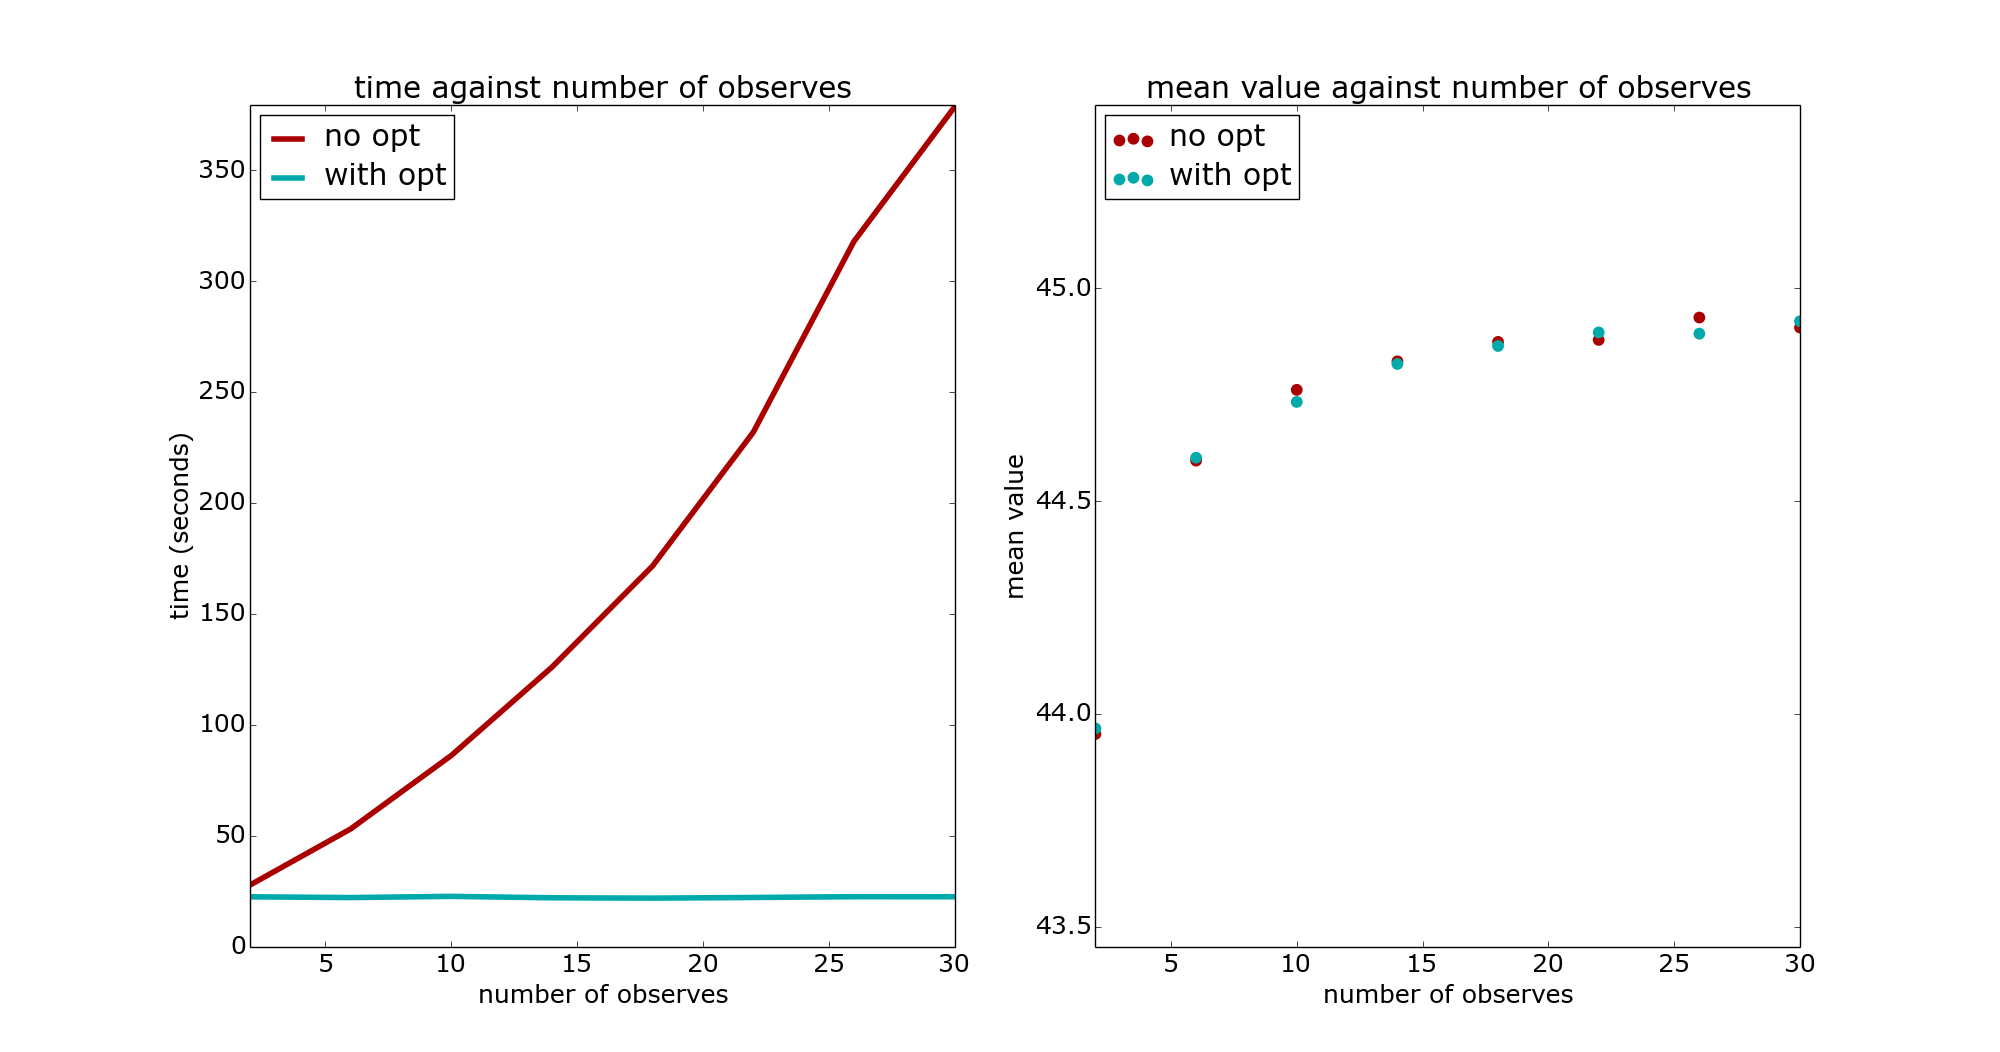
\includegraphics[width=16cm]{images/merging_observes_1.png}}

What you can see from these is firstly that the optimized and non-optimized programs give the same answer. Also, the optimized program is far faster. Considering the computational complexity it appears that the non-optimized program is close to linear in the number of observes, but the optimized program running time remains constant.

I will now investigate the \(n = 30\) case in more detail. These aspects can be seen in the following two graphs. The first graph shows the final posterior distribution. The second graph shows how the mean varies over time. The value at \(t\) is the mean of the first \(t\) iterations.

\centerline{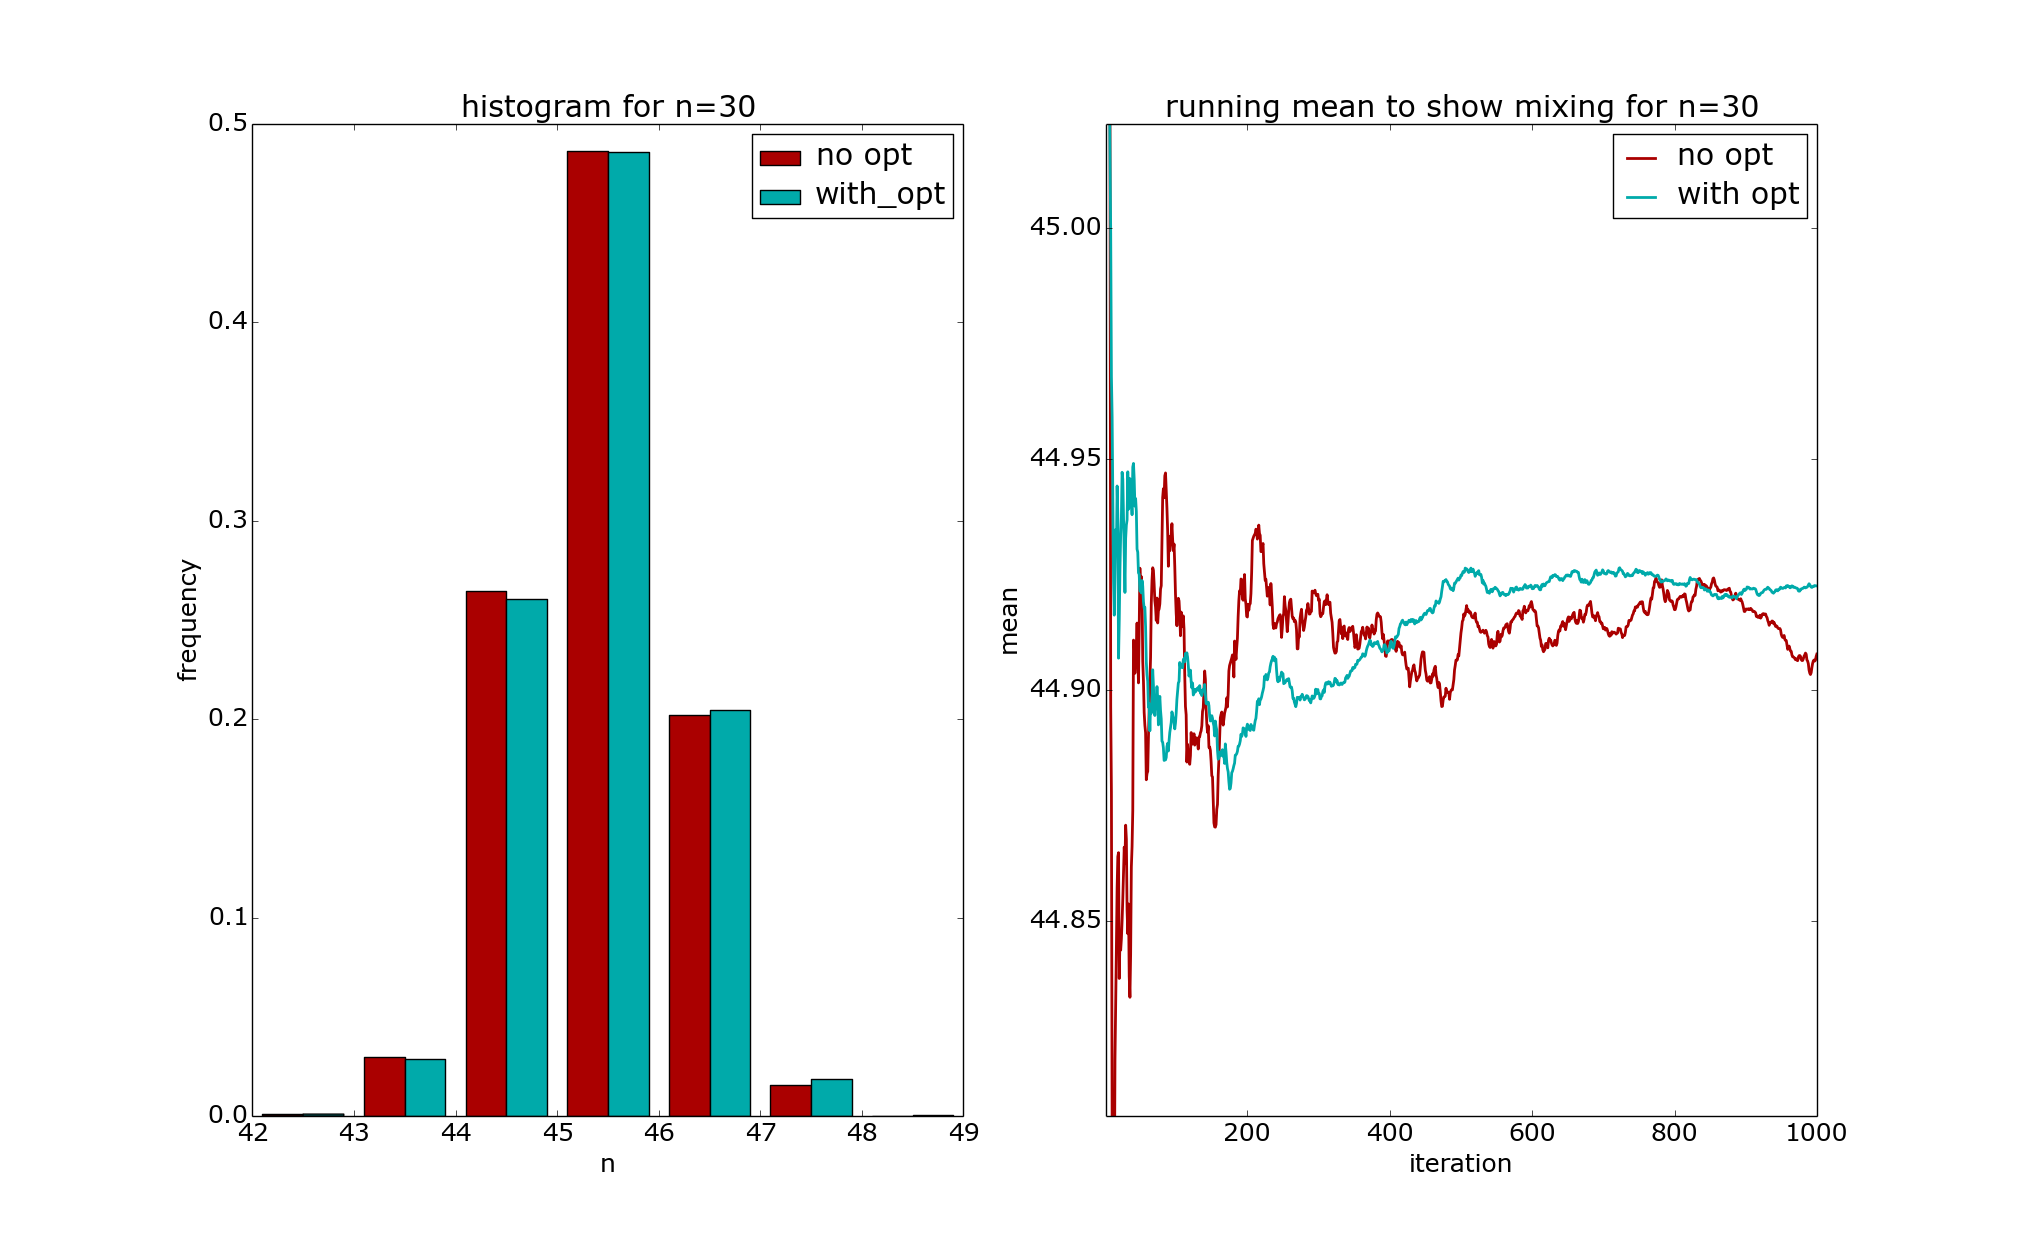
\includegraphics[width=16cm]{images/merging_observes_2.png}}

What you see from the first graph is again that the optimized and non-optimized programs give the same answer. Looking at the second graph it appears that the optimized program reaches it's final answer after around 600 iterations whilst the non-optimized program has still not converged satisfactorily after 1000 iterations. At first glance the optimized program has better mixing, however I don't feel this is conclusive and would instead say that they perform roughly equally.



%    ########       ###### 
%    ##            ##    ##
%    ##                  ##
%     ######        ###### 
%          ##            ##
%    ##    ##  ##  ##    ##
%     ######   ##   ###### 

\subsection{Merging any consecutive observes}

To test this optimization I used a program of the following form.

\[
	\begin{array}{l}
		\texttt{[assume m (normal 5 1)]} \\
		\texttt{[assume f (lambda () -> Num m)]} \\
		\texttt{[observe (normal (f) 0.1) 4]} \\
		\texttt{...} \\
		\texttt{[observe (normal (f) 0.1) 4]} \\
		\texttt{[predict m]}
	\end{array}
\]
Where the number of observe statements was varied. Programs of the above form were compiled with either no optimizations enabled or all optimizations enabled, then the resulting programs were run for 1000 iterations with 100 particles.

The following two graphs show running time against number of observes and mean value of the posterior distribution against number of observes.

\centerline{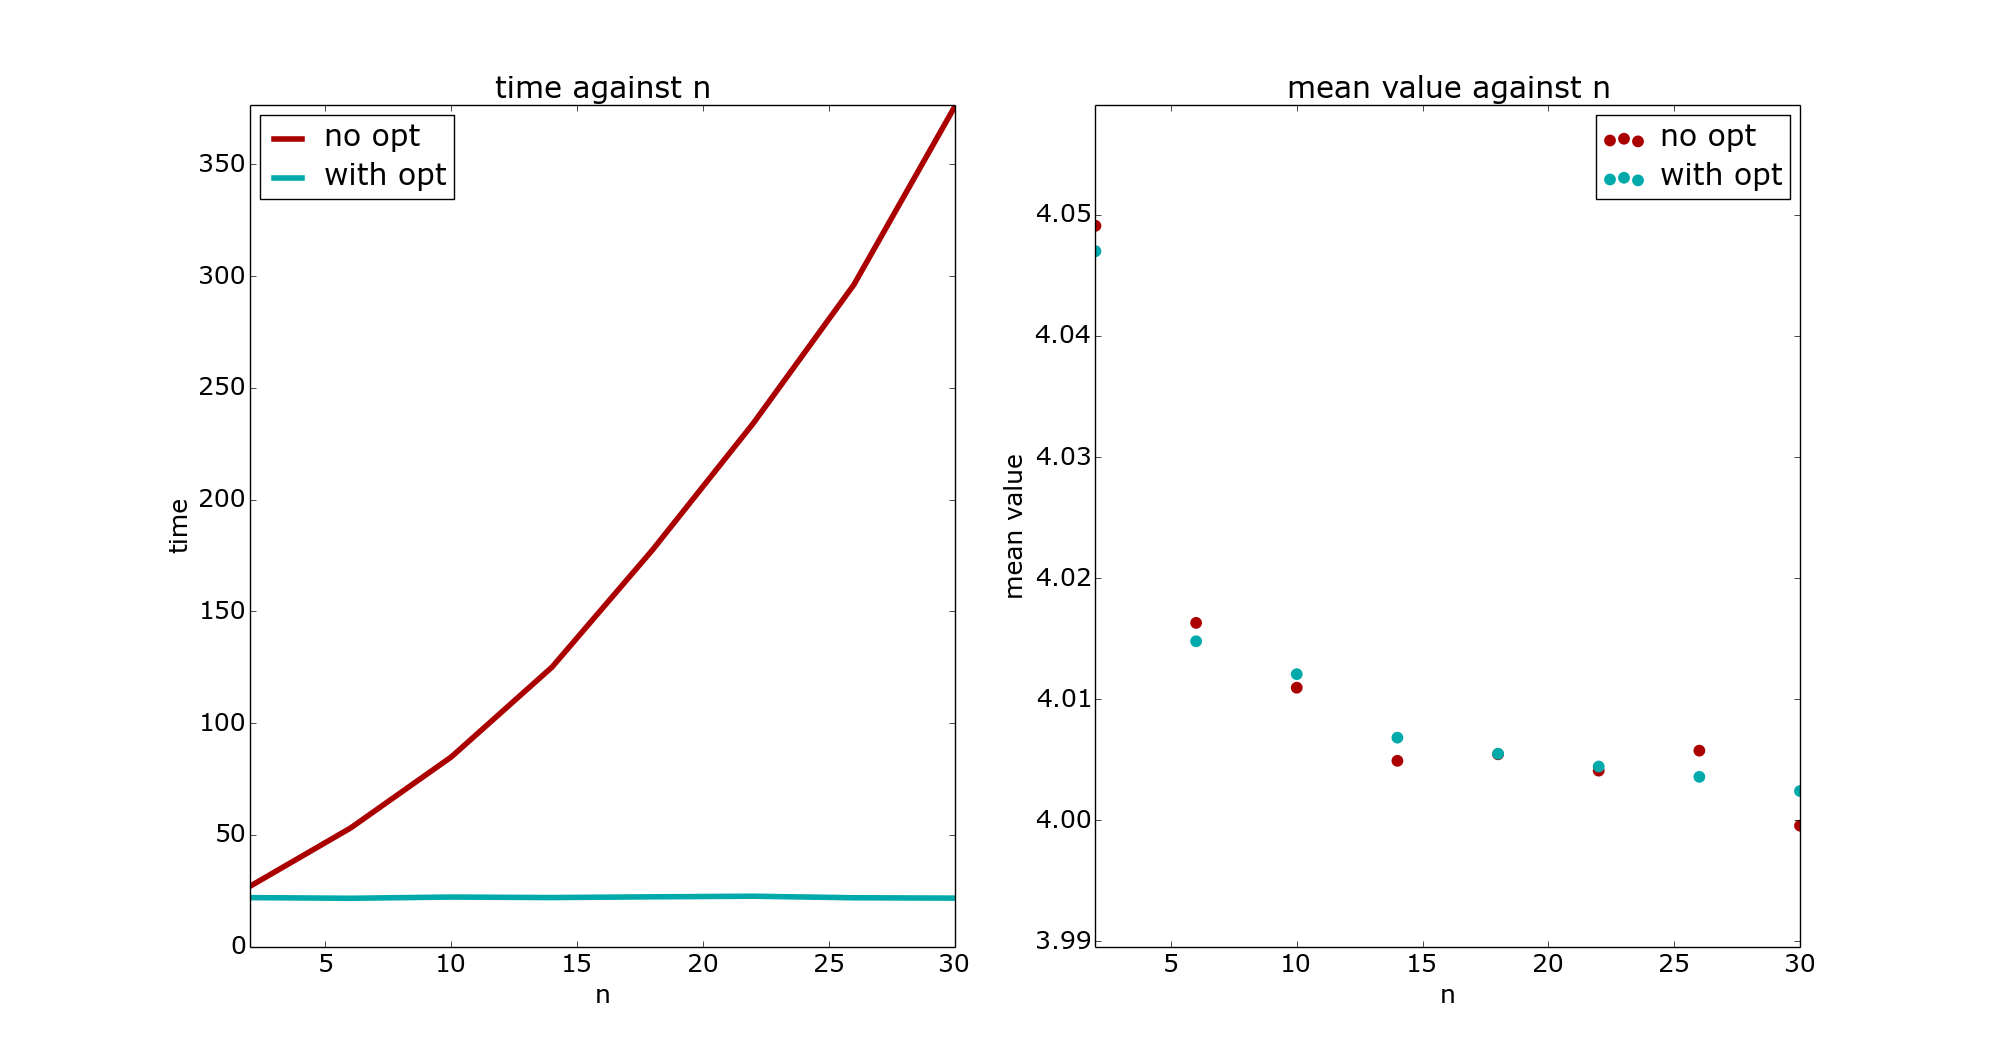
\includegraphics[width=16cm]{images/merging_consecutive_observes_1.png}}

What you can see from these is firstly that the optimized and non-optimized programs give the same answer to within an acceptable margin, but again that the optimized program is far faster. Considering the computational complexity it again appears that the non-optimized program is close to linear in the number of observes, however the optimized program running time remains constant.

I will now investigate the \(n = 30\) case in more detail. These aspects can be seen in the following two graphs. The first graph shows the final posterior distribution. The second graph shows how the mean varies over time, so the value at t is the mean of the first t iterations.

\centerline{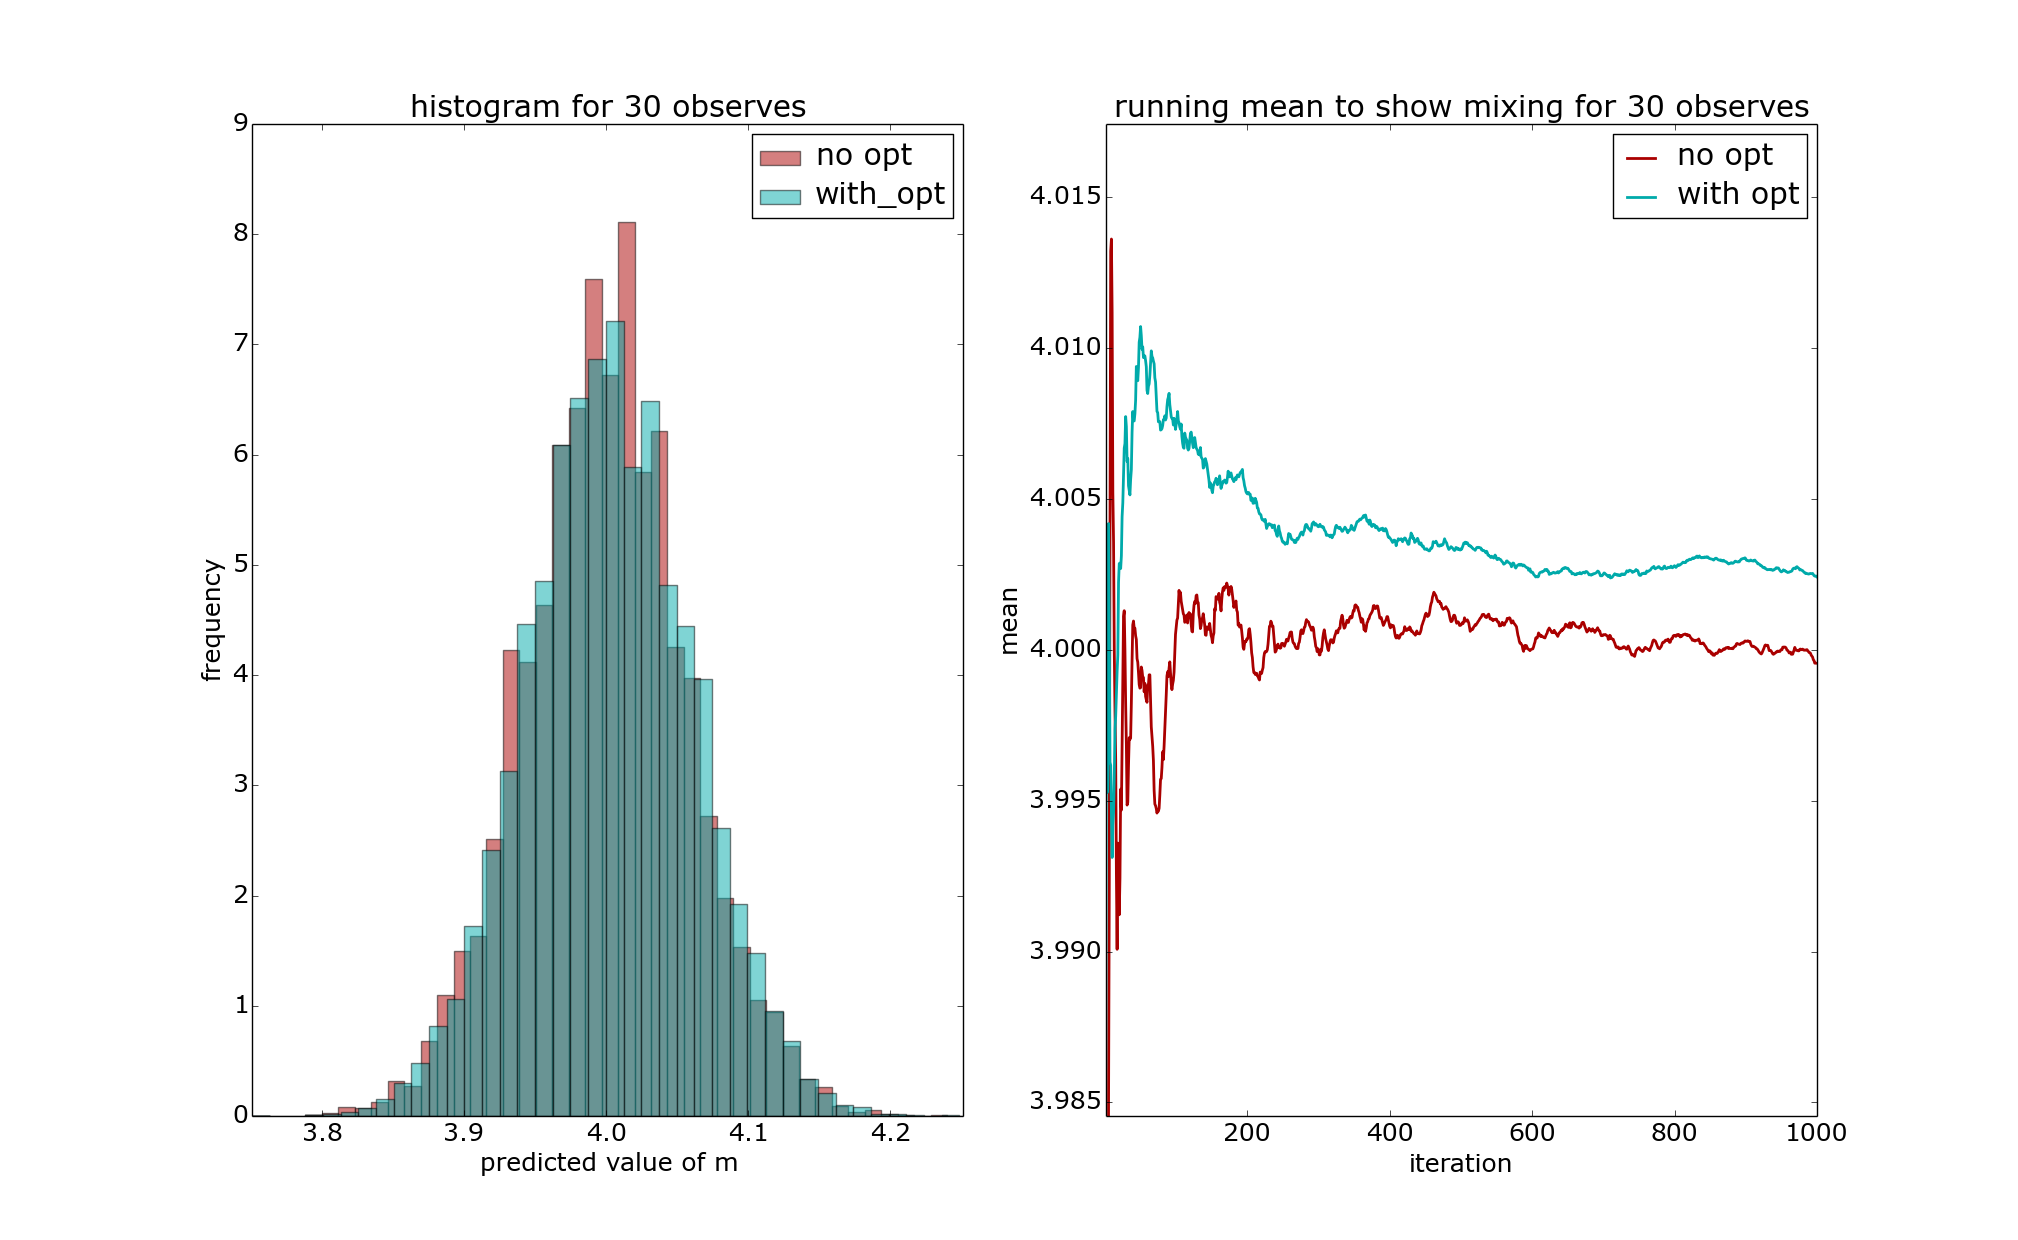
\includegraphics[width=16cm]{images/merging_consecutive_observes_2.png}}

What you see from the first graph is again that minus a bit or noise the optimized and non-optimized programs give the same answer. Looking at the second graph they appear to have similar levels of mixing. They both approach their final mean value of posterior distribution at the same rate.



%    ########          ### 
%    ##               #### 
%    ##              ## ## 
%     ######        ##  ## 
%          ##      ########
%    ##    ##  ##       ## 
%     ######   ##       ## 

\subsection{Removing observes}

To test this optimization I used a program of the following form.

\[
	\begin{array}{l}
		\texttt{[assume m (normal 10 4)]} \\
		\texttt{[observe (normal m 0.1) 15]} \\
		\texttt{...} \\
		\texttt{[observe (normal m 0.1) 15]} \\
		\texttt{[predict m]}
	\end{array}
\]
Where the number of observe statements was varied. Programs of the above form were compiled with either no optimizations enabled or all optimizations enabled. The resulting programs were then run for 1000 iterations with 100 particles.

The following two graphs show running time against number of observes and mean value of the posterior distribution against number of observes.

\centerline{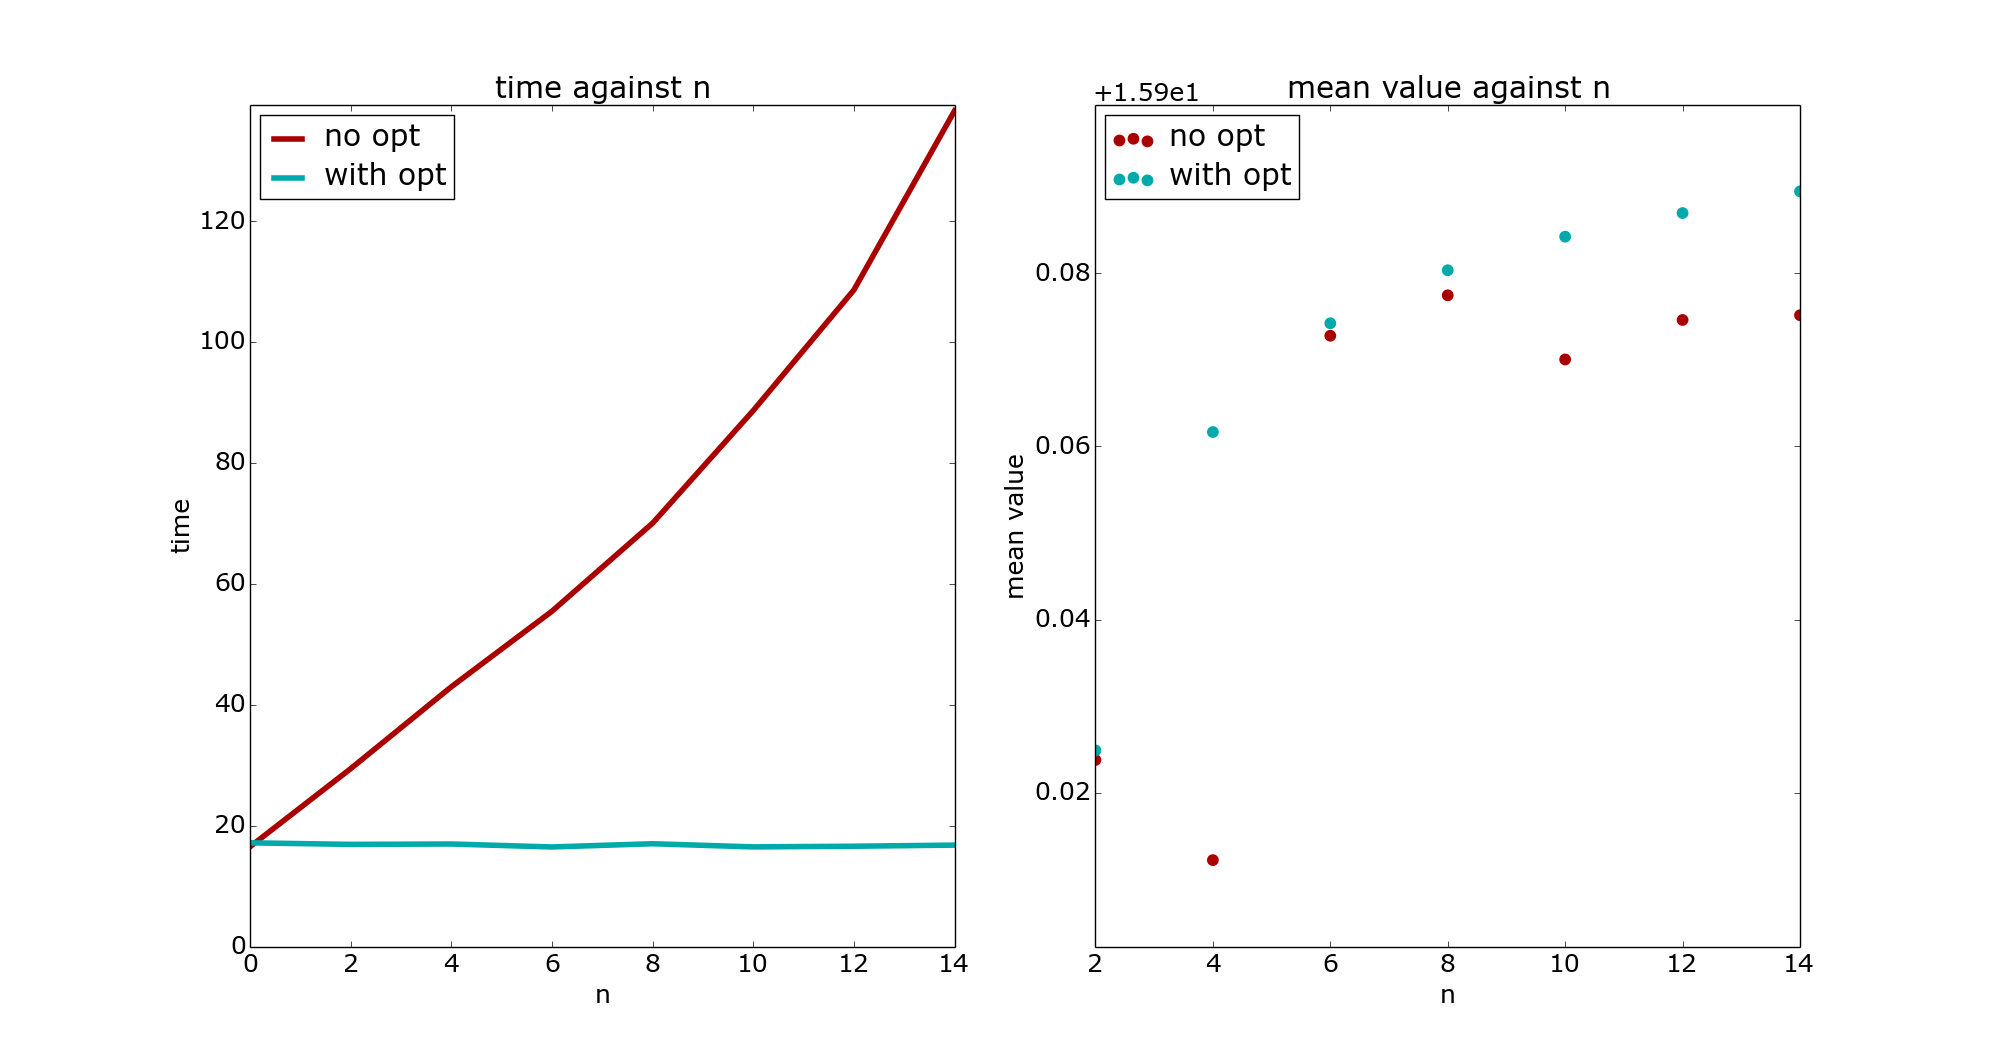
\includegraphics[width=16cm]{images/removing_observes_1.png}}

What you can see here is firstly that the optimized program is far faster than the non-optimized one, but the optimized program gives a sensible and correct answer whereas the non-optimized programs are much less consistent. Considering computational complexity it again appears that the non-optimized program is close to linear in the number of observes, however the optimized program running time remains constant.

I will now show the extend to which the non-optimized programs fail to give usable output. Looking at the posterior distribution of each one and showing how it deteriorates as the number of observes increases. Consider the following set of graphs.

\centerline{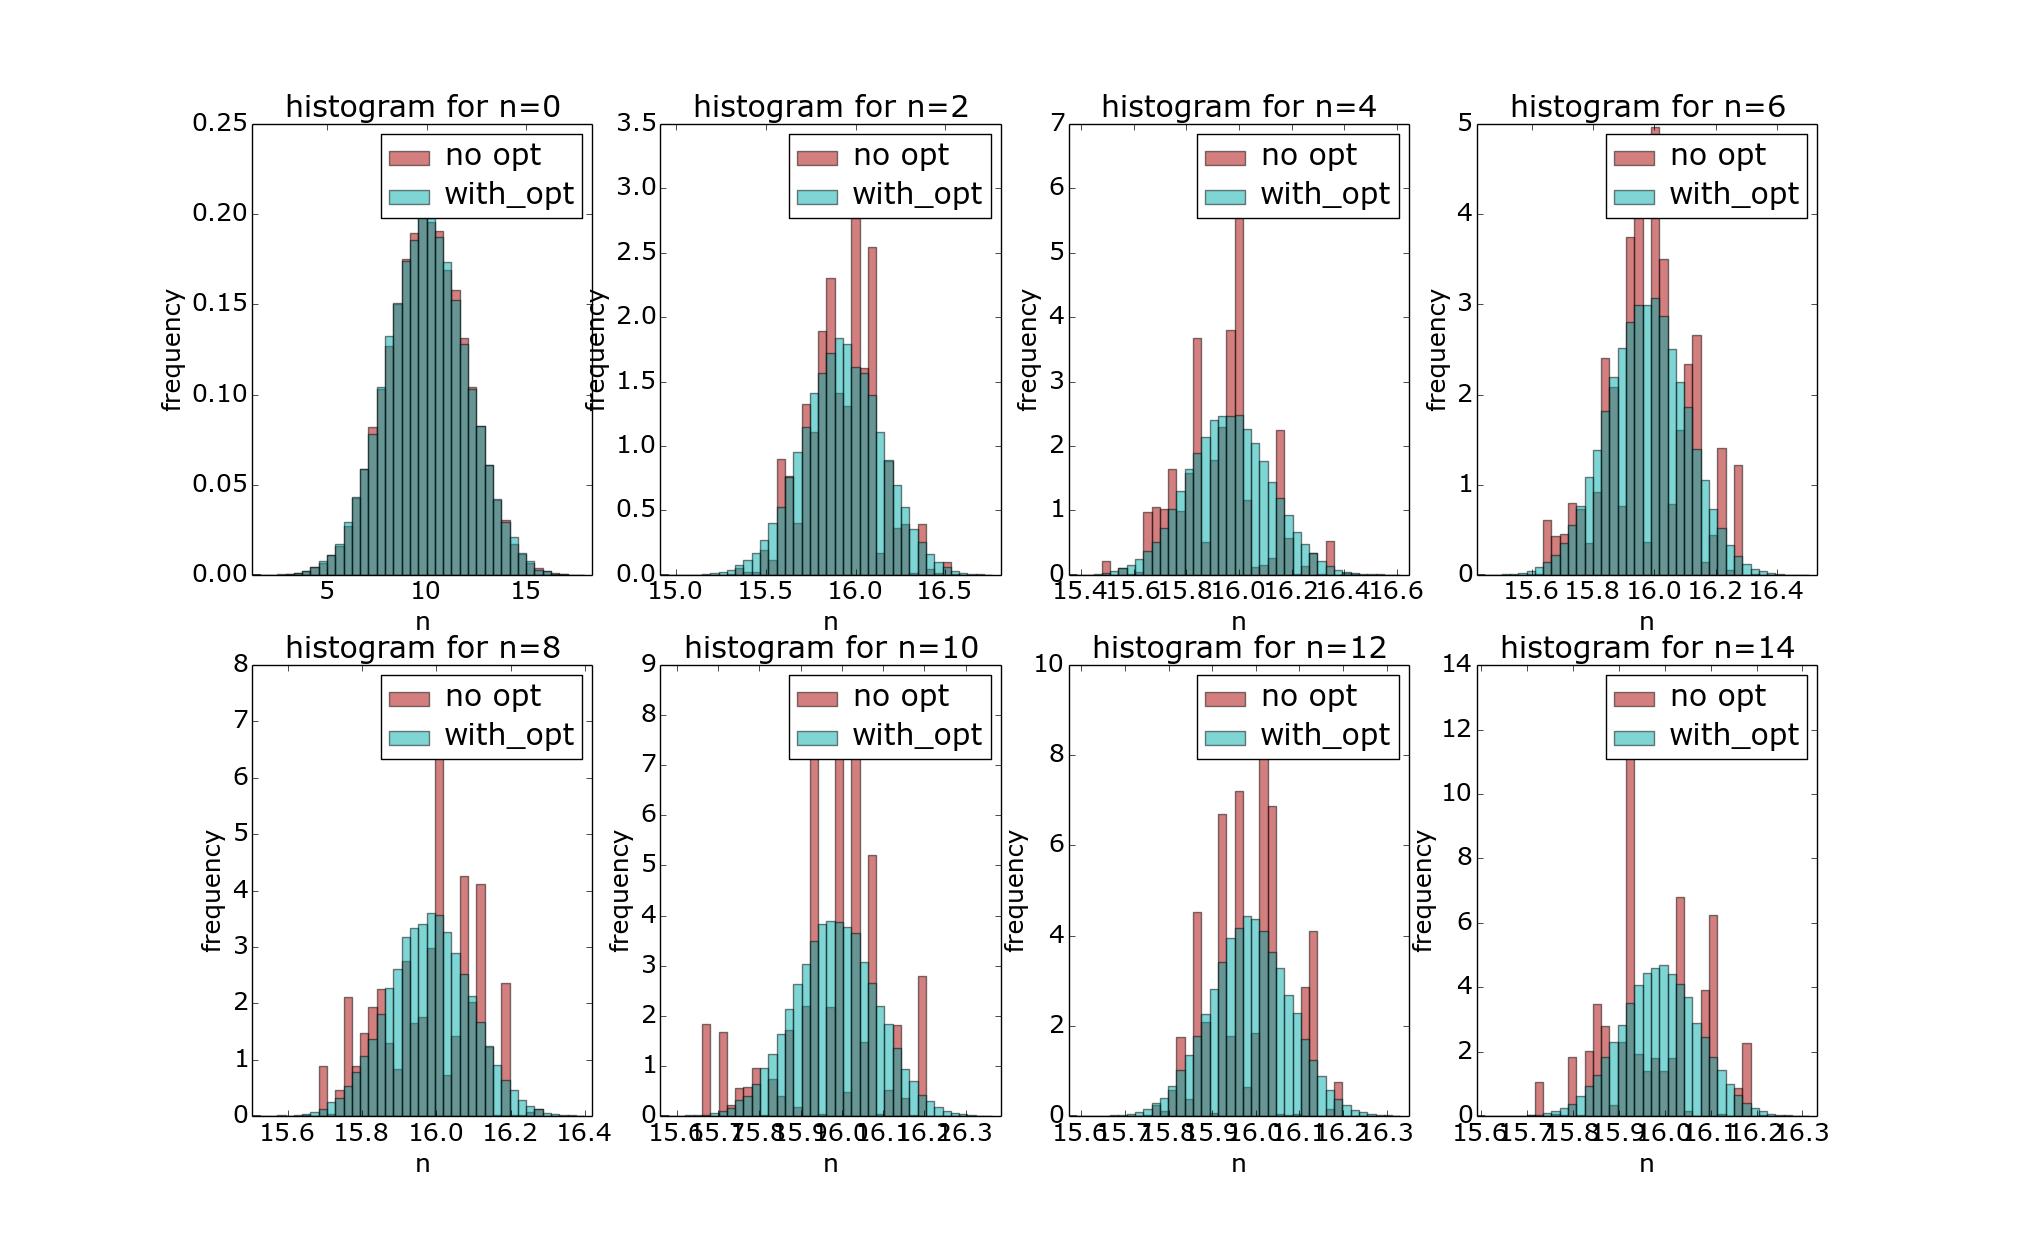
\includegraphics[width=16cm]{images/removing_observes_2.png}}

What you can see here is that the optimized program gives a perfect normal distribution every time. In fact we could have run far fewer than 1000 iterations and still achieved a good distribution. However, the non-optimized program's distributions are much less clean and if we were to increase the number of observes more or move the observed value further from the value \texttt{m} then the distributions would deteriorate even more. The non-optimized program is not even usable except in easy cases. This optimization actually opens whole new areas of program that can be written rather than just making things faster.



%    ########      ########
%    ##            ##      
%    ##            ##      
%     ######        ###### 
%          ##            ##
%    ##    ##  ##  ##    ##
%     ######   ##   ###### 

\subsection{Removing constant observes}

To test this optimization I used the following program.

\[
	\begin{array}{l}
		\texttt{[assume x (uniform-continuous 0 1)]} \\
		\texttt{[observe (flip 0.5) true]} \\
		\texttt{[predict x]}
	\end{array}
\]
Where the point is that the optimization would remove the observe and change nothing else. The above program was compiled with either no optimizations enabled or all optimizations enabled. The resulting programs were then run for 1000 iterations with 100 particles.

The result on speed was that the optimized program was approximately 27\% faster. When counting the number of unique samples in an iteration, the non-optimized program had on average 47\% unique samples, but the optimized program had on average 63\% unique samples. What we see here is that removing a constant observe improves the program in all ways.



%        ##       ####### ##    ## ######## ##    ## ######   #######      ##          ##  #####  ######   ##   ##
%       ##    ##  ##      ##    ##    ##    ##    ## ##   ##  ##           ##          ## ##   ## ##   ##  ##  ## 
%      ##     ##  ##      ##    ##    ##    ##    ## ##   ##  ##            ##   ##   ##  ##   ## ##   ##  ## ##  
%     #####       #####   ##    ##    ##    ##    ## ######   ######        ##  ####  ##  ##   ## ######   ####   
%    ##   ##  ##  ##      ##    ##    ##    ##    ## ##  ##   ##             ####  ####   ##   ## ##  ##   ## ##  
%    ##   ##  ##  ##      ##    ##    ##    ##    ## ##   ##  ##             ####  ####   ##   ## ##   ##  ##  ## 
%     #####       ##       ######     ##     ######  ##    ## #######         ##    ##     #####  ##    ## ##   ##

\section{Future work}

We have had various idea for ways that the compiler could be improved upon. Most of these ideas are small and are just things that we did not have time to implement initially. Some ideas however would require more work and large changes throughout the compiler.

\begin{itemize}
\item
	We only implemented a small number of optimizations from each category. For example we only implemented the optimization to reduce multiple observes from the same family to one observe for the normal distribution. This optimization could be made for many other distribution families and it would be interesting to implement it for more of them. The optimization dealing with conjugate prior distributions could also be done for more distributions than we originally had time for. In all cases we expect the relationship has already been discovered by mathematicians and we only need to peruse the subject matter to find all the relationships of interest. This was not done due to time constraints.

\item
	Reducing arithmetic in the outputted C code would have no to little effect on the speed of the program but would be interesting to do and make the outputted C code smaller and prettier. This is something already done by compilers. Due to Anglican using only floating point numbers and no integers the transformations will be slightly easier than if it did. We did not implement this due to time constraints and the fact that it is of little use.

\item
	Currently any if statement in the source program results in a continuation in the final C program. Each continuation increases complexity and is slow to execute. In many cases however it would be possible to get away without a continuation. This would involve using standard compiler techniques and is not hugely interesting. It was not implemented originally because of the difficulty of the transformations.

\item
	The source language G currently has extra type information. It would be nice to be able to remove this and use unaltered Anglican as our source language. This would consist of two parts as type information is used in two places.

	The extra information in function types could be removed by doing standard, well understood analysis to infer the type or infer that no type could possibly work. For functions that are then called with multiple different but possible types we may have to create one function in the outputted C code for each type used. This is the way that C++ templating works.

	When extracting items from lists we currently use extra type information to know what we're expecting and then halt execution if we receive something different. The benefit of doing it this way is that we can use native C types once we've extracted the value. The down side is of course that extra type information is needed. The way to fix this would be to not use native types but extract into a data structure that holds one variable from a selection of types. Doing this would allow us to more closely model the semantics of Lisp. It is not clear what the performance penalty would be.

	The reason that both of these extra features were not added is because they are difficult to implement and not necessary to demonstrate the optimizations. If this system were to be extended to a usable one however then we would have to look at these as we would want to use an unmodified existing untyped language such as Anglican as the source language.

\item
	There is a feature of Anglican and of many other probabilistic and traditional programming languages called memoization. This feature caches the results of a function. Normally this is only used for performance reasons. In a probabilistic programming language memoization is used to cache the output of probabilistic functions and this allows one to write a whole new class of model. An example of a new model that could be written is probabilistically generating an automaton that accepts a set of words. Anglican has a primitive \texttt{mem} which turns a normal function into a cached one. Probabilistic-C also provides an implementation of caching so threading them together shouldn't be too difficult. The reason this was not done originally is because of time constraints and the difficulty of making sure that the two implementations of caching are identical in their semantics.

\item
	There is an issue that for very simple programs Probabilistic-C can be slower than the original Anglican. Generally if the program does not involve user-defined functions then Anglican will execute significantly faster. However, when more complicated features are involved such as user-defined functions and lists the generated Probabilistic-C comes out as faster. There are a few hypothesis that it would be interesting to test out. It could be to do with the compilation introducing unnecessary continuations which slow down execution. It could be because of Probabilistic-C's high use of multi-threading and my test computer is not suited to fast execution. Whatever the reason it would be nice to make it faster if possible.

\end{itemize}



%    ########       #####   #####  ##    ##  #####  ##     ##    ##  #####  ####  #####  ##    ##
%         ##   ##  ##   ## ##   ## ###   ## ##   ## ##     ##    ## ##       ##  ##   ## ###   ##
%        ##    ##  ##      ##   ## ####  ## ##      ##     ##    ## ##       ##  ##   ## ####  ##
%       ##         ##      ##   ## ## ## ## ##      ##     ##    ##  #####   ##  ##   ## ## ## ##
%      ##      ##  ##      ##   ## ##  #### ##      ##     ##    ##      ##  ##  ##   ## ##  ####
%     ##       ##  ##   ## ##   ## ##   ### ##   ## ##     ##    ##      ##  ##  ##   ## ##   ###
%    ##             #####   #####  ##    ##  #####  ######  ######   #####  ####  #####  ##    ##

\section{Conclusion}

What we have achieved in this project is to create an optimizing compiler from a high level Lisp based probabilistic programming language to a lower level C based probabilistic programming language. The compilation itself is interesting enough although we did have to add extra type information to the source language to make the compilation easier. However, the real aim of the compiler was to perform various probabilistic optimizations during compilation. Optimizations we apply include merging multiple samples from one distribution family into one sample, merging together multiple observes from the same family, merging any consecutive observes, and potentially completely removing observes when they form a conjugate prior.

Overall we think that the project has been a success. The compiler compiles source code successfully and the although the performance improvement varies by program it can be up to 50 percent. There is then in general at least one probabilistic optimization that can be applied to any program and this produces both huge speed increases and improvements to the quality of samples generated. By leveraging the optimizations it becomes possible to write entire classes of model that before were infeasible. It would be more impressive if unaltered Anglican were used as the source language but we explain in the previous section that although this is possible there just was not time to implement it.

We hope that this project can be continued to produce a system that could feasibly be used in production. Along with other research we are confident that the efficiency of probabilistic programming systems will continue to improve. We only hope that this project is a step in that direction and benefits other researchers.



\bibliography{g2c}{}
\bibliographystyle{plainurl}

\end{document}
